%FJERDE KAPITLET.


\chapter{Det naturliga urvalet.}
{\it
Det naturliga urvalet; dess verksamhet jemförd med menniskans urval; dess verkan på egenskaper af ringa vigt; dess verksamhet på alla åldrar och kön. — Sexuelt urval. — Om allmänheten af kroasering emellan individer af samma art. Gynsamma och ogynsamma omständigheter för det naturliga urvalet, isynnerhet kroasering, isolering, antal af individer. — Långsam verkan. — Tillintetgörelse genom det naturliga urvalet. — Karakterens divergens med afseende på inbyggarnas olikhet inom ett litet område, och på naturalisering. — Det naturliga urvalets verkan på afkomlingar af gemensamma föräldrar genom karakterens divergens och genom tillintetgörelse. — Förklarar alla organiska varelsers gruppering. — Framåtskridande i organisation. — Bibehållandet af ofullkomliga former. — Invändningar. — Oinskränkt förökning af arter. — Sammanfattning.
}\\[0.5cm]

Denna kamp för tillvaron, som vi i förra kapitlet allt för kort afhandlat, hvilka verkningar kan den åstadkomma med afseende på föränderligheten? Kan principen om urvalet, så mäktig i menniskans hand äfven tillämpas i naturen? Vi skola se, att dess verkningar i naturen äro utomordentliga. Vi måste ihågkomma, i huru ändlöst antal af besynnerligheter våra kulturalster visa variationer och äfven naturens alster ehuru i mindre grad, och huru stark benägenheten hos dessa variationer är att gå i arf. Men den föränderlighet, som vi nästan öfverallt bland våra kulturalster påträffa, är såsom Hooker och Asa Gray riktigt anmärka, icke direkt menniskans verk; hon kan hvarken framkalla nya variationer, ej heller förhindra deras uppkomst, hon kan blott bibehålla dem som erbjudas henne och föröka dem. Utan beräkning försätter hon de organiska varelserna under förändrade lefnadsvilkor och variationerna begynna. Men likartade omvexlingar i lefnadsförhållandena kunna äfven förekomma i naturen och förekomma der äfven. Vi måste också ihågkomma, i huru oändligt inveckladt förhållande alla lefvande varelser stå till hvarandra, huru de lämpa sig efter hvarandra och efter de naturliga lefnadsförhållandena och hvilken oändlig mängd bildningsförändringar kunna gagna hvarje varelse under vexlande lifsvilkor. Om man ser, huru många för menniskan nyttiga variationer otvifvelaktigt förekomma, kan man då anse det för osannolikt, att under loppet af tusentals generationer andra variationer förekomma, mer eller mindre fördelaktiga för hvarje varelse i den stora och invecklade kampen för tillvaron? Men om sådana förekomma, kunna vi då ännu tvifla, att de individer (då flera individer födas, än som kunna fortlefva) som hafva någon om ock ringa fördel öfver de andra hafva största sannolikheten att öfverlefva de andra och fortplanta sin typ? Å andra sidan kunna vi med visshet antaga, att en variation som är det minsta skadlig är hemfallen till undergång. Detta bibehållande af fördelaktiga och förkastande af ofördelaktiga variationer är hvad jag kallar det naturliga urvalet. Förändringar, som äro hvarken nyttiga eller skadliga lemnar det naturliga urvalet orörda, och de blifva qvar såsom ett vacklande element, sådant vi måhända se det i de så kallade polymorfa arterna eller blifva slutligen fixa, alltefter organismens och lifsvilkorens beskaffenhet.

Man har missförstått uttrycket det naturliga urvalet eller funnit det olämpligt. Några hafva till och med ansett, att det naturliga urvalet leder till föränderlighet, då det likväl blott föranleder sådana förändringars bestånd, som för organismen äro af nytta under dess egendomliga lefnadsförhållanden. Ingen förebrår landbrukaren, att han talar om de stora verkningar menniskans urval åstadkommit, och i detta fall måste de individuela egendomligheter, som menniskan med ett visst mål i sigte väljer till fortplantning, först hafva förekommit i naturen. Andra hafva gjort den invändningen, att ordet val förutsätter ett medvetet väljande hos djuren, som undergå förändringarna; man har till och med framhållit, att växterna icke hafva någon vilja och derföre skulle uttrycket icke kunna användas på dem. Otvifvelaktigt är uttrycket i bokstaflig bemärkelse oriktigt, men hvem klandrar kemisten derför att han talar om sina elementers valfrändskap, men icke kan man i egentlig mening säga, att en syra väljer sin bas för att förena sig med. Man har sagt, att jag talar om det naturliga urvalet såsom om en gudomlig makt, men hvem kan förebrå någon, att han talar om attraktionen som styr planeternas rörelser? Hvar menniska vet hvad som menas med dessa bildliga talesätt, de äro för korthetens skull nödvändiga. Det är lika svårt att undvika en personifiering af ordet natur, men med natur menar jag blott de förenade verkningarna och resultaten af det stora antalet naturlagar, och med naturlagar fenomenens kända successiva uppträdande. Sådana ytliga invändningar hafva ingen vigt för den som gjort sig litet förtrogen med det vetenskapliga språket.

Det sannolika förloppet vid det naturliga urvalet inse vi lätt, om vi fästa oss vid ett specielt fall, ett land som undergått någon fysisk förändring till exempel i klimatet. Proportionerna af inbyggarnas antal skola omedelbart förändras och en eller annan art skall helt och hållet dö ut. Inbyggarna på en trakt stå vidare, såsom vi hafva sett, i ett intimt och inveckladt beroende af hvarandra, och deraf kunna vi sluta, att oberoende af klimatets förändringar olikheten i antal af en del af invånarna äfven skall hafva ett väsentligt inflytande på de öfriga. Har landet öppna gränser, skola säkerligen nya former invandra och äfven detta skall märkbart störa förhållandet emellan de gamla invånarna; vi erinra oss, hvilka stora följder införandet af en enda trädart eller däggdjursart haft i de ofvan meddelade exemplen. Hade vi deremot för oss en ö eller ett delvis naturligen inhägnadt och afstängdt land, så att nya och mera passande former i större antal ej kunde tränga in på området, så skulle vi i naturens hushållning finna luckor, som skulle bättre fyllas af på vederbörligt sätt modifierade individer af de ursprungliga invånarna, ty hade landet varit öppet för inflyttning, så skulle de nykomna hafva fyllt dessa luckor. Hvarje liten afvikelse, som under tidernas lopp utvecklat sig och på något sätt gynnat individerna af den ena eller andra arten, skulle i detta fall hafva utsigt att ega bestånd och det naturliga urvalet hafva fritt spelrum för sitt förbättringsarbete.

Såsom vi hafva visat i första kapitlet, hafva vi goda skäl för det antagandet, att en förändring i lefnadsomständigheter förorsakar eller förökar föränderligheten hufvudsakligen genom sitt inflytande på det reproduktiva organsystemet. I det fall vi nu tänkt oss hafva vi antagit en förändring i de yttre omständigheterna, och detta skall säkerligen vara gynsamt för det naturliga urvalet derigenom att sannolikheten för nyttiga variationers uppträdande på samma gång blifvit större, och om icke några nyttiga variationer förekomma, kan naturen icke göra något val. Dertill behöfves visst icke någon ansenligare grad af föränderlighet, ty på samma sätt som menniskan kan vinna stora resultat genom att samla blott individuela olikheter i en och samma riktning, så står detta äfven i naturens förmåga, det är för henne blott mycket lättare, då hon har ojemförligt mycket längre tid till sin disposition. Ej heller tror jag, att någon stor fysisk förändring till exempel i klimat, eller en ovanlig grad af isolering till skydd för inflyttning är nödvändig för bildandet af nya och outfyllda luckor, som det naturliga urvalet bör fylla genom modifiering och förbättring af några varierande inbyggare. Ty då alla invånarna i hvarje trakt med väl afvägda krafter ligga i en beständig kamp med hvarandra, så äro ofta ytterst små afvikelser i bygnad eller lefnadsvanor tillräckliga att gifva en invånare någon öfvervigt, så länge han lefver under samma förhållanden och begagnar samma näringsmedel och försvarsmedel. Man kan icke uppgifva någon trakt, i hvilken alla naturliga invånare så fullkomligt passa för hvarandra och för de yttre förhållanden under hvilka de lefva, att icke någon af dessa skulle kunna förädlas, ty i alla trakter äro de inhemska produkterna till den grad besegrade af naturaliserade alster, att de hafva låtit dessa främlingar taga landet definitivt i besittning. Och då främlingarna öfverallt hafva tillintetgjort en del af de infödda, så kunna vi utan fruktan draga den slutsatsen, att de öfriga undergått några fördelaktiga modifikationer, så att de bättre kunnat göra motstånd mot inkräktarna.

Då menniskan genom sitt omedvetna eller metodiska urval kunnat vinna sådana resultat, hvad skall då icke naturen kunna åstadkomma? Menniskan kan blott verka på synliga och yttre karakterer; naturen, om det tillåtes att personifiera det naturliga bibehållandet af föränderliga och gynnade individer under kampen för tillvaron, naturen frågar icke efter utseendet, såvida det icke kan vara nyttigt för ett visst ändamål. Hon kan verka på hvarje inre organ, på den minsta skilnad i organisation, på hela lifsmaskineriet. Menniskan väljer blott för sin egen nytta, naturen blott för den varelses nytta, som hon skyddar; hvarje af henne utvald karakter bibehålles derföre i full verksamhet och varelsen försättes under gynsamma yttre omständigheter. Menniskan håller på samma ställe individer födda i flera klimat och låter sällan en karakter blifva verksam på något särskildt och passande sätt, hon sätter lång- och kortnäbbade dufvor på samma kost, hon använder ett långryggigt och ett långbent däggdjur till samma arbete, och utsätter kortulliga och långulliga får för samma klimat. Hon låter icke den kraftfullare hannen sjelf tillkämpa sig sin hona, hon förstör icke alltid de ofullkomligare djuren, utan skyddar snarare alla sina produkter, så mycket i hennes makt ligger, under hvarje årstid. Ofta börjar hon sitt urval med en till hälften monströs form eller åtminstone med en mera framstående variation, som fängslar hennes öga eller lofvar henne någon synbar fördel. I naturen deremot kan redan den minsta afvikelse i kroppsbygnad vara nog att upphäfva den jemvigt som hittills egt rum emellan de kämpande formerna och härigenom vinna bestånd. Huru vexlande äro icke menniskornas önskningar och sträfvanden, huru kort är hennes lif och huru torftiga äro icke hennes produkter i jemförelse med dem, som naturen samlat under loppet af hela geologiska perioder! Böra vi då förundra oss öfver, att naturprodukterna hafva en vida mer äkta karakter än menniskans, att de vida bättre passa för de mest invecklade lefnadsvilkor och bära prägeln af ett vida högre mästerskap?

I figurlig mening kan man säga, att det naturliga urvalet är dagligen och stundligen sysselsatt öfver hela verlden med att pröfva hvarje variation äfven den obetydligaste, förkastande hvad som är dåligt och behållande och förbättrande det som är godt, stilla och obemärkt, alltid och allestädes der tillfälle erbjudes arbetande på fulländandet af hvarje organisk varelse med afseende på dess organiska och oorganiska lefnadsvilkor. Vi se intet af dessa långsamma förändringar till framåtskridande, förrän tidens finger visar på en förlupen verldsperiod, och då är vår blick i de längesedan förflutna geologiska perioderna så otillräcklig, att vi ingenting annat se, än att lifsformerna nu äro helt andra än de varit.

För att en högre grad af modifikation under århundradens lopp skall kunna uppkomma, är det nödvändigt, att en varietet, en gång bildad, ånyo varierar om också först efter en längre period, och att dess variationer bibehållas om de äro goda, och så vidare. Ingen naturhistoriker skulle väl vilja neka, att varieteter stundom förekomma, som mer eller mindre afvika från föräldrarnas stamform; men att denna förvandlingsprocess skulle kunna fortgå i oändlighet, det är ett antagande hvars riktighet måste bedömas efter dess öfverensstämmelse med de allmänna naturföreteelserna och efter dess förmåga att förklara desamma. Den vanliga åsigten, att föränderligheten icke kan öfverskrida en viss gräns, hvilar lika väl blott på ett antagande.

Ehuru det naturliga urvalet blott kan verka i och för hvarje varelses bästa, så beröras deraf äfven egenskaper och bildningar, som vi blott kunna tillägga en underordnad vigt. Om vi finna bladätande insekter gröna, barkätande gråspräckliga, fjellripan om vintern hvit, om vi se, att skotska ripan har ungefär hedens färg, orren torfmossens, så hafva vi skäl att antaga, att sådana färger äro nyttiga för de nämda insekterna och fåglarna och tjena dem till skydd. Om riporna icke under någon period af sitt lif voro utsatta för ödeläggelse, så skulle de föröka sig till oändligt antal; de äro utsatta för förföljelse af roffåglar, som upptäcka sitt byte med sin skarpa syn; i vissa trakter af Europa har man varnat för hvita dufvor, emedan de så lätt bli rof för sina fiender. Derföre synes det mig icke tvifvel underkastadt, att det just är det naturliga urvalet, som förlänat hvarje art af ripa eller orre dess egendomliga färg och bibehållit den äkta och oförfalskad, då den en gång blifvit förvärfvad. Vi få icke heller tro, att en tillfällig förstöring af ett djur med en viss färg har blott en ringa påföljd; vi erinra oss, huru vigtigt det är att ur en hvit fårahjord afskilja hvarje lam, som visar blott det ringaste spår af svart. Vi hafva förut sett, att i Florida färgen på svinen, som äta en viss rot, bestämmer öfver deras lif och död. Botanister räkna fjunet på frukterna och färgen på fruktköttet till de minst vigtiga kännetecken, och dock få vi höra af en utmärkt trädgårdsodlare, Downing, att i Förenta Staterna de nakna frukterna lida mera skada än de håriga af en skalbagge, en Curculio, och att röda plommon äro mera utsatta för en viss sjukdom än de gula, under det en annan sjukdom vida oftare angriper de gula persikorna än andra. Om under användande af alla konstens medel dessa obetydliga olikheter kunna bestämma öfver odlandet af vissa varieteter, så är det säkert, att i naturtillståndet, då träden hafva att kämpa med andra träd och med en mängd fiender, sådana olikheter verksamt deltaga i bestämmandet af de varieteter som skola bibehållas, de glatta eller håriga, de gula eller röda frukterna.

Om vi tänka på en mängd små olikheter emellan arter, som vi anse för oväsentliga, så vidt vår okunnighet tillåter oss att döma, så få vi icke förgäta, att äfven klimat, näring och andra omständigheter kunna hafva en direkt verkan. Men det är vida nödvändigare att komma ihåg, att det finnes många ännu obekanta lagar för utvecklingens vexelverkan, hvilka, om en del af organisationen modifieras genom variation och om dessa modifikationer af det naturliga urvalet samlas till varelsens bästa, föranleda andra modifikationer, ofta af det mest oväntade slag.

De förändringar som i kulturtillståndet uppträda på en viss bestämd period af lifvet visa sig gerna, såsom vi hafva sett, äfven hos afkomman på samma period, — till exempel förändringar i form, storlek och smak på fröna af många köks- och åkerväxter, i larverna och kokongerna af våra silkesmaskvarieteter, i äggen af våra fjäderfä och i ungarnas dunbeklädnad, i hornen på våra nötkreatur och får, då de äro nära fullväxta, — och på samma sätt eger äfven i naturtillståndet det naturliga urvalet förmåga att verka på och modifiera de organiska varelserna i en viss ålder, derigenom att det samlar förändringar som äro gagneliga för denna ålder och låter dem gå i arf i en viss lifsperiod. Om det för en växt är af nytta, att dess frön allt mer och mer kringspridas af vinden, så kan jag icke se någon större svårighet för det naturliga urvalet att åstadkomma detta, än för bomullsodlaren att genom urval föröka och förbättra bomullen i frökapslarna af hans växter. Det naturliga urvalet kan modifiera en insektlarv och göra den passande för många förhållanden, fullkomligt olika de omständigheter, under hvilka den fullt utbildade insekten framdeles kommer att lefva och dessa förändringar skola säkerligen enligt lagarna för vexelverkan hafva något inflytande på den fullmogna insektens bygnad. Så kunna efter all sannolikhet äfven vissa förändringar hos den fullmogna insekten tvärtom inverka på larvens bygnad, men i alla händelser skall det naturliga urvalet sörja för, att de modifikationer som blott äro följder af modifikationer under en annan lifsperiod icke äro skadliga för djuret, emedan de då skulle hafva till följd artens utslocknande.

Det naturliga urvalet kan modifiera ungarnas bildning i förhållande till föräldrarna och föräldrarnas i förhållande till barnen. Bland djur som lefva i samhällen gör urvalet hvarje individs skapnad lämplig för samhället, på samma gång som individen sjelf har fördel af den valda modifikationen. Hvad det naturliga urvalet ej kan åstadkomma är en arts förändring till sin nackdel, till förmån för en annan art, och ehuru i naturhistoriska arbeten exempel derpå anföras, kan intet af dem hålla streck vid en noggrannare pröfning. Till och med en sådan organisk bildning, som blott en gång i djurets lif användes, kan om den för djuret är af stor vigt af det naturliga urvalet modifieras till huru hög grad som helst, såsom några insekters stora käkar, hvilka blott tjena till kokongernas öppnande, eller den hårda spetsen på unga fåglars näbb, som blott användes till äggskalets brytning. Man påstår med visshet, att af de bästa kortnäbbade tumletterna flera gå under i ägget än som kunna krypa ut, en sak som gifver dufamatörer anledning att hjelpa till vid skalets brytning. Om nu naturen hade för afsigt att göra en dufvas näbb mycket kort till dufvans egen fördel, så skulle denna process gå mycket långsamt för sig, och dervid måste samtidigt ske det noggrannaste urval af de unga fåglar, som i ägget hafva starkaste och hårdaste näbben, emedan alla med mjuk näbb oundvikligen skulle omkomma; eller ock skulle ett urval ske af de tunnaste och lättast brutna skal, hvilket också som bekant varierar lika väl som hvarje annan bildning.



\section{Sexuelt urval.}

I kulturtillståndet uppträda ofta egendomligheter hos ett visst kön och hålla sig ärftliga inom samma kön och sannolikt sker detsamma äfven i naturtillståndet; om detta är förhållandet, så måste det naturliga urvalet vara i stånd att modifiera ett kön i dess funktionella förhållande till det andra könet eller i vanor, som sålunda blifva mer eller mindre olika hos båda könen, hvarpå man ej sällan finner exempel hos insekter, och detta ger mig anledning att säga några ord om hvad jag kallar sexuelt urval. Detta urval beror icke på en kamp för tillvaron utan en kamp emellan hannarna om besittningen af honan, och resultatet af striden är icke den svagare kämpens död, utan en obetydligare eller alls ingen afkomma af honom. Det sexuela urvalet är derföre mindre strängt än det naturliga urvalet. De kraftigaste hannarna, som bäst fylla sin plats i naturen, lemna i allmänhet det största antalet afkomlingar. Men i många fall beror utgången af striden icke på styrkan i allmänhet, utan på vissa vapen, som kommit hannen allena till del. En hornlös hjort och en tupp utan sporre hafva ringa utsigt att efterlemna någon afföda. Ett sexuelt urval, som ständigt ger segraren möjligheten af fortplantning, måste förse tuppen med ett okufligt mod, långa sporrar och starka vingar för att låta honom med större kraft använda sin beväpnade fot; på samma sätt som en brutal handlande med stridstuppar vet att genom sorgfälligt urval förädla sina djur i detta hänseende. Huru långt ned i naturens skala dylika strider förekomma, vet jag icke; man har berättat om alligatorhannar, huru de kämpa om en hona, vråla och svänga rundt likt indianer i en stridsdans; laxhannar har man stundom sett strida med hvarandra dagen i ända, och hannarna af ekoxen bära ofta sår af andra starkare ekoxars käkar; den såsom observator ojemförlige Fabre såg hannarna af vissa steklar kämpa om en hona, som satt bredvid såsom overksam åskådare af striden och sedermera åtföljde segraren. Striden är måhända häftigast emellan hannarna af sådana djur som lefva i polygami och dessa tyckas i allmänhet vara försedda med särskilda vapen dertill. Rofdjurshannen är redan i och för sig väl beväpnad, dock plägar det sexuela urvalet gifva både dem och andra djur särskilda försvarsvapen, såsom lejonets man, laxhannens hakformiga underkäk, ty skölden är väl för krigaren lika vigtig som svärdet och spjutet.

Bland fåglarna är giljarestriden ofta af en mera fredlig karakter. Alla som sysselsätta sig med denna fråga hafva kommit till den åsigten, att rivaliteten emellan sångfåglarnas hannar yttrar sig häftigast i sången, med hvilken de locka till sig sina honor. Klipptrasten i Guiana, paradisfågeln och några andra samla sig i skaror och hannarna utbreda den ena efter den andra sin ståtliga fjäderbeklädnad och intaga de mest besynnerliga ställningar för honan, som står bredvid såsom åskådare och slutligen väljer den behagligaste friaren. Noggranna iakttagare af fåglar i fångenskap veta väl, att de ofta visa starkt utpräglade sympatier och antipatier för vissa individer; sir R. Heron har beskrifvit huru en skäckig påfågelhanne var särdeles omtyckt af alla hans honor. Jag kan här icke ingå på alla detaljer, som vore nödvändiga för att styrka min åsigt; men om en menniska är i stånd att på kort tid gifva sina bantamhöns en elegant hållning och skönhet efter sitt begrepp om skönhet, så kan jag ej finna tillräckligt skäl till tvifvel, att fågelhonan också kan åstadkomma en märkbar förändring genom att under tusentals generationer gifva företräde åt den melodirikaste eller skönaste hannen efter hennes begrepp om skönhet. Jag anser möjligt, att några väl kända lagar för hannars och honors fjäderbeklädnad i jemförelse med ungarnas låta förklara sig efter den åsigt, att fjäderbeklädnaden hufvudsakligen modifieras genom det sexuela urvalet, som verkar då fåglarna hunnit könsmognad eller under fortplantningstiden. De derpå beroende förändringarna gå derföre i arf på motsvarande ålder och årstid antingen på hannen eller på hannen och honan; men jag har här icke tillfälle att närmare inlåta mig på detta ämne.

Om derföre hanne och hona hafva samma lefnadsvanor i allmänhet, men i skapnad, färg eller prydnad afvika från hvarandra, så bero dessa olikheter enligt min tanke hufvudsakligen på det sexuela urvalet; det vill säga manliga individer hafva under flera på hvarandra följande generationer haft någon liten fördel öfver andra i vapen, försvarsmedel eller tjusningskraft och dessa fördelar hafva gått i arf på deras manliga afkomlingar. Dock vill jag icke härleda alla sådana könsolikheter från samma ursprung, ty vi se hos hannarna af våra husdjur egendomligheter uppträda och hålla sig ärftliga hvilka vi icke kunna antaga vara af nytta för hannen under strid eller utöfva någon dragningskraft på honan, såsom hudvårtorna hos den engelska brefdufvan, de hornartade utväxterna hos några hannar af hönsfåglarna och flera dylika. Analoga fall se vi också i naturtillståndet, till exempel hårtofsen på bröstet hos kalkonen, som hvarken kan vara ett vapen i striden eller någon prydnad, och skulle denna tofs hafva bildat sig först under tama tillståndet, skulle vi kalla den en monstrositet.



\section{Exempel på det naturliga urvalet.}

För att göra klart, på hvad sätt i min tanke det naturliga urvalet verkar, måste jag med läsarens benägna tillåtelse gifva ett eller två tänkta exempel. Vi tänka oss först en varg, som lefver af åtskilliga djur, som han förskaffar sig dels genom list, dels genom styrka och dels genom snabbhet, och vi antaga, att hans snabbaste byte, hjorten till exempel, af någon orsak hade på någon trakt i hög grad förökat sig, eller att andra till dess näring tjenliga djur hade förminskats på de tider då vargen hade svårt att förskaffa sig föda. Under sådana förhållanden synes det mig klart, att de smärtaste och snabbaste vargarna hafva största utsigten att blifva vid lif och sålunda blifva skyddade och utvalda, förutsatt likväl, att de på samma gång bibehålla nog styrka att bemäktiga sig sitt byte äfven på en annan tid, då de kunde tvingas att uppsöka andra djur till sin föda. Detta synes mig lika sannolikt, som att menniskan kan föröka sina vindthundars snabbhet genom sorgfälligt och metodiskt urval eller genom detta omedvetna urval, som uppkommer af hvar och ens bemödanden att förskaffa sig de bästa hundarna utan hvarje tanke på rasens förädling. Jag bör tillägga, att i Catskillbergen i Förenta Staterna finnas två vargvarieteter enligt Pierce, en af en smärt vindthundlik form, som förföljer hjortar, och en annan mera tjock med korta ben, som oftare angriper fårahjordarna.

Man måste iakttaga, att jag i ofvanstående exempel talat om de smärtaste vargindivider och icke om någon särskild, väl markerad variation. I de tidigare upplagorna af detta arbete yttrade jag mig såsom om detta senare alternativ ofta hade inträffat. Jag såg den stora vigten af individuela olikheter och detta föranledde mig att afhandla resultaten af menniskans omedvetna urval, som beror på bevarandet af de mest passande och värdefullaste individer och tillintetgörandet af de odugliga. Jag såg också, att bevarandet i naturtillståndet af en tillfällig afvikelse, såsom en monstrositet, skulle vara en sällsynt händelse, och att, om den bibehölls, den skulle i allmänhet förloras genom följande kroasering med vanliga individer. Förr än jag hade läst en värderik artikel i ”North British Review” (1867), insåg jag likväl icke, huru sällan enstaka variationer, vare sig obetydliga eller väl utpräglade, kunna ega bestånd. Författaren antager exemplet af ett par djur, som under sin lifstid alstra tvåhundra afkomlingar, af hvilka inalles blott två till följd af olika orsaker fortlefva för att fortplanta sitt slägte. Detta är visserligen en ytterlighet för de flesta högre djur men alldeles icke för många af de lägre organismerna. Han visar vidare, att om en enda individ föddes, som varierade på något vis och derigenom fick två gånger så stora utsigter för lifvet som de andra djuren, så vore dock faran för dess lif stor. Antaget att den lefde och lemnade afföda, och att hälften af dess efterkommande ärfde den gynsamma variationen, så skulle, såsom författaren visar, afkomlingarna hafva blott ringa utsigt att blifva i lif och fortplanta sig, och denna utsigt skulle fortfarande förminskas under de följande generationerna. Riktigheten af dessa anmärkningar kan såsom jag tror icke bestridas. Om till exempel en fågel af något slag kunde få sin föda på lättare vis derigenom att den hade krökt näbb, och om en sådan föddes med ovanligt stark krökning på näbben, och som följaktligen frodades, så vore det likväl ringa utsigt för denna enda individ att fortplanta sin form och utrota den vanliga; men af hvad vi se under domesticering skall detta otvifvelaktigt blifva följden af ett under flera generationer fortsatt bibehållande af ett stort antal individer med mer eller mindre böjda näbbar och ett utrotande af ett ännu större antal individer med de rakaste näbbarna.

Man får likväl icke förbise, att vissa variationer, hvilka ingalunda kunna betraktas såsom blott individuela skiljaktigheter, ofta uppkomma derigenom att likartade organisationer utsättas för likartade inflytelser — och härpå kunna gifvas talrika exempel bland våra kulturalster. I sådana fall om en varierande individ icke verkligen öfverflyttar på sin afkomma sin nyförvärfvade karakter, skall den dock otvifvelaktigt, så länge de förhandenvarande förhållandena äro desamma lemna honom en ännu starkare benägenhet att variera på samma sätt. Lefnadsförhållandena böra verka så energiskt och bestämdt, att de leda till samma modifikation hos alla individer af arten utan allt biträde af urvalet. Men vi kunna antaga, att förhållandena räckte till att verka på blott en tredjedel, fjerdedel eller tiondedel af individerna; och flera sådana exempel kunde gifvas; så har Grabo till exempel visat, att på Färöarna omkring en femtedel af grislorna, som alla lägga ägg tillsammans, består af en väl markerad varietet, som fordom upptogs såsom en särskild art under namn af Uria lacrymans. Om i sådana fall variationen vore fördelaktig, skulle den ursprungliga formen snart undanträngas af den modifierade enligt grundsatsen om de bäst utrustade rasernas bestånd.

Med afseende på verkningarna af kroasering och konkurrens måste vi hålla i minnet, att de flesta djur och växter hålla sig vid sina egna hem och icke onödigtvis vandra omkring; vi se detta just ibland flyttfåglar, hvilka nästan alltid återvända till samma plats. Följaktligen bör hvarje nybildad varietet i allmänhet först vara lokal, hvilket synes vara den allmänna regeln med varieteter i naturtillståndet; så att lika modifierade individer snart skola uppstå på ett litet område och ofta yngla tillsammans. Om den nya varieteten var lycklig i striden för tillvaron, skall den småningom sprida sig från en central fläck, kämpande med och besegrande de oförändrade individerna på gränserna af en alltid tillväxande cirkel. Men till kapitlet om kroasering skola vi återkomma. De som icke sysselsatt sig med naturalhistoria kunna invända, att ett länge fortsatt hopande af individuela olikheter icke skall kunna gifva upphof till delar och organer som synas oss och stundom kallas nya. Men såsom vi hädanefter skola finna är det svårt att framtaga ett exempel på ett verkligen nytt organ; ett så inveckladt och fulländadt organ som ögat kan visas sjunka ned till en enkel väfnad med känslighet för diffust ljus.

Låt oss nu taga ett mera inveckladt fall. Vissa växter afsöndra en söt vätska, tydligen för att aflägsna något ofördelaktigt ur deras saft. Hos många leguminoser sker detta genom körtlar vid basen af stiplerna och hos den vanliga lagern på bladens rygg. Denna vätska, om den också finnes blott i ringa mängd, uppsökes med begärlighet af insekter. Vi antaga, att en blomma afsöndrar litet sådan söt saft eller nektar vid basen af kronbladens insida. Insekterna som uppsöka denna saft skulle i detta fall blifva beströdda med pollenkorn och säkerligen ofta öfverföra dem från en blomma till en annans pistill. Blommorna af två skilda individer af en art blifva på detta sätt kroaserade och kroaseringen lemnar (såsom vi hafva skäl att tro och hvartill vi framdeles återkomma) en särdeles kraftig afföda, som följaktligen har mesta sannolikhet att fortlefva och fortplanta sig. Några af dessa efterkommande skola med all säkerhet ärfva denna afsöndringsförmåga och de blommor som hafva de största glandlerna och lemna mesta nektarn uppsökas helst af insekterna och blifva oftast kroaserade med hvarandra, och skola på detta sätt under tidernas lopp taga öfverhand. De blommor, som hafva sina ståndare och pistiller så placerade i förhållande till storleken och andra egendomligheter hos de insekter som besöka dem, att öfverflyttandet af pollenkornen från en blomma till en annan underlättas, de blifva på samma sätt favoriserade och utvalda. Om vi antaga, att insekterna ville samla pollenkornen i stället för nektar, så skulle detta vara en förlust för blomman, då frömjölet alstras blott till växtens befruktning; dock, om litet frömjöl af de samlande insekterna bortfördes, i början händelsevis och sedermera af vana, och öfverfördes från en blomma till en annan, skulle den härigenom uppkomna kroaseringen vara till stor nytta för växten, om också nio tiondedelar af frömjölet förstördes; och de växtindivider, som producerade mera frömjöl och hade större ståndare, blefvo naturligen utvalda.

Om nu våra växter genom denna process af fortsatt naturligt urval af de mest eftersökta blommorna hafva för våra insekter blifvit särdeles behagliga, så skola dessa, å sin sida fullkomligt utan afsigt, regelbundet transportera frömjöl från blomma till blomma, och att de i detta hänseende kunna vara ytterst verksamma, kunde jag bevisa genom många slående exempel. Till bevis vill jag blott anföra ett fall, icke såsom mycket slående, men emedan det tillika kan tjena såsom ett exempel på ett steg till könens åtskilnad hos växterna, hvarom vi strax skola tala. Några jernekar frambringa blott hanblommor, som innehålla fyra ståndare med en temligen ringa mängd frömjöl och en förkrympt pistill; andra lemna blott honblommor, som hafva en fullständigt utbildad pistill och fyra ståndare med förkrympta ståndarknappar, i hvilka ej ett enda pollenkorn kan upptäckas. Jag fann ett träd med honblommor på sextio alnars afstånd från ett hanträd; ur tjugu blommor från skilda grenar tog jag märkena, lade dem under mikroskopet och i dem alla utan undantag upptäckte jag några pollenkorn och på några till och med en oerhörd mängd deraf. Då vinden under flera dagar hade gått i riktning från det honliga trädet till hanträdet, så kunde frömjölet icke med vindens tillhjelp kommit i honblommorna. Vädret hade under några dagars tid varit kallt och blåsigt, och derföre ogynsamt för bien, och det oaktadt var hvarje af mig undersökt honblomma befruktad genom bin med pollenkorn, som bien under sitt sökande efter nektar från blomma till blomma hade med sina hår fört från hanträdet hitöfver. Men låt oss återvända till det fall vi tänkt oss; så snart denna växt blifvit för insekterna särdeles tilldragande, så att de regelbundet föra frömjölet från en blomma till en annan, inträder en annan process. Ingen vetenskapsman tviflar på fördelen af hvad man kallar arbetets fysiologiska fördelning; derföre kan man tro, att det för en växtart är fördelaktigt, att i en blomma eller på en hel individ alstras blott ståndare och i en annan blomma eller på en annan individ blott pistiller. Hos odlade växter och sådana som blifvit försatta under nya lefnadsförhållanden felslå ofta de hanliga och någon gång de honliga organerna. Antaga vi att detta sker i naturtillståndet i aldrig så ringa grad, så skulle individer med en mer eller mindre utvecklad tendens dertill fortfarande favoriseras och utväljas, tills slutligen könen voro fullständigt skilda, emedan frömjölet sedan regelbundet transporteras från blomma till blomma och könens fullständiga skiljande är för dem fördelaktig enligt principen om arbetets fördelning. Det skulle upptaga för mycket utrymme att visa de olika vägar, genom dimorfism eller andra medel, hvarpå könens särskiljande hos växter af olika arter nu fortskrider. Emellertid vill jag till det ofvan anförda tillägga, att enligt Asa Gray i Nordamerika finnas några jerneksarter på ett mellanstadium, hvilkas blommor äro såsom, den nämda botanisten uttrycker sig, mer eller mindre dioecistiskt-polygama.

Vi skola nu återvända till våra af nektar lefvande insekter i det fall vi tänkt oss; vi antaga att växten, hvars nektarbildning vi hafva sett långsamt förökas genom ett fortgående naturligt urval, är en allmän art och att vissa insekter äro hänvisade hufvudsakligen till dess nektar såsom föda. Genom flera exempel skulle jag kunna visa biens bemödanden att inbespara tid; jag vill blott anföra deras vana att hacka hål i botten af vissa blommor för att komma åt deras nektar, som de med litet mera möda kunde hemta upp ur blommornas mynningar. Med dessa fakta för ögonen tror jag mig kunna antaga, att en tillfällig afvikelse i kroppsstorlek och form, i längd och krökning af snabeln, om ock alltför obetydlig att af oss kunna iakttagas, kunde för ett bi eller en annan insekt vara af en sådan nytta, att en så utrustad individ vore i stånd att lättare förskaffa sig sin föda och härigenom hade mer utsigt att blifva vid lif och lemna afföda efter sig. Hans afkomlingar skulle sannolikt få i arf en benägenhet till en likartad obetydlig afvikelse i samma organ. De rörformiga blomkronorna af Trifolium pratense (vanlig rödklöfver) och Tr. incarnatum synas vid ett flyktigt betraktande icke afvika mycket i längd från hvarandra; det oaktadt kunna honing- eller kupbien (Apis mellifica) lätt suga nektarn ur den sednare, ej ur den röda, som derföre uppsökes blott af humlor; hela fält af rödklöfver erbjuda derföre förgäfves bien ett öfverflöd af dyrbar nektar. Att bien tycka mycket om denna nektar är säkert, ty jag har flera gånger ehuru blott om hösten sett många af dessa bin suga nektarn genom hål som humlorna hade bitit vid basen af blomkronan. För bien vore det derföre en stor fördel att hafva en något längre eller på annat sätt formad snabel. Å andra sidan har jag såsom ofvan är nämdt genom försök funnit, att rödklöfverns fruktbarhet till största delen beror på de honingsökande bien, hvilka under denna sysselsättning rubba blommans delar ur sitt läge och på detta sätt öfverföra frömjölet på pistillens märke. Olikheten i längden af de båda klöfverarternas blomkrona måste vara obetydlig, ty man har försäkrat mig, att om rödklöfvern slås, blifva blommorna af de nya skotten något mindre och besökas talrikt af bin. Jag vet icke om denna uppgift är riktig, ej heller om ett annat meddelande är tillförlitligt, att de liguriska bien, som i allmänhet blott anses för en varietet af de vanliga bien och rikligen kroaseras med dem, att de hafva förmågan att komma åt den vanliga rödklöfverns nektar och uppsuga den. I en trakt, der denna klöfverart rikligen förekommer kan det derföre för honingbien vara af stor nytta att hafva en något längre eller något olika formad snabel. Men å andra sidan, då denna klöfvers fruktbarhet absolut beror på att någon biart rubbar kronbladen ur sitt läge, så skulle, om humlorna på en trakt blefvo sällsynta, en kortare eller djupare delad blomkrona vara för rödklöfvern af största nytta, så att honingbien skulle kunna besöka dess blommor. På detta sätt kan jag förstå huru en blomma och ett bi småningom, vare sig samtidigt eller den ena efter den andra, kunna modifieras och lämpas efter hvarandra på det fullkomligaste sätt genom de individers bestånd, som å ömse sidor förete obetydliga bildningsafvikelser, gynsamma för begge.

Jag vet väl, att den genom föregående tänkta exempel förklarade satsen om det naturliga urvalet är utsatt för samma inkast som Ch. Lyell’s storartade åsigter i ”the modern changes of the earth, as illustrative of Geology”; emellertid höra vi numera sällan de ännu verksamma orsakerna kallas obetydliga och ringa, då de tillämpas på urhålkandet af de djupaste dalar eller på bildandet af långa sträckor af fastlandsklippor. Det naturliga urvalet kan blott verka genom ett samlande af oändligt små ärfda modifikationer, som alla för varelsen äro fördelaktiga; och på samma sätt som den nyare geologien för det mesta har bannlyst sådana åsigter, som stora dalars urhålkande genom en enda diluvialström, på samma sätt skall äfven det naturliga urvalet, om det är riktigt, bannlysa tron på en fortsatt skapelse af nya organiska varelser eller på stora och hastiga modifikationer i deras bildning.



\section{Om individers kroasering.}

Här måste jag göra en liten digression. Det är klart, att af djur och växter med skilda kön måste för hvarje befruktning tvänne individer förenas, med undantag af de märkvärdiga och ännu ej förklarade fallen af Parthenogenes. Men hvad hermafroditerna beträffar är detta långt ifrån uppenbart. Det oaktadt är jag mycket benägen att tro, att af alla hermafroditer, antingen i allmänhet eller ock vid vissa tillfällen, tvänne individer samverka för artens fortplantning. Denna åsigt har förut blifvit framstäld af Andrew Knight och vi skola straxt se dess vigt; denna fråga kan jag visserligen blott vidröra i största korthet, men jag har rikligt material samladt för en utförligare behandling. Alla ryggradsdjur, alla insekter och dessutom några andra större djurgrupper para sig för hvarje befruktning. Nyare undersökningar hafva betydligt förminskat antalet förr antagna hermafroditer och af de verkliga hermafroditerna para sig många, det vill säga, två individer förena sig regelbundet till hvarandras befruktning, och detta är allt som vi här behöfva taga i betraktande. Det gifves dessutom många andra hermafroditiska djur, som vanligen icke para sig, och det allra största antalet växter äro hermafroditiska. Hvad finnes, kan man fråga, i detta fall för skäl till det antagandet, att för hvarje gång två individer samverka vid befruktningen? Då det här icke är möjligt att ingå på enskildheter, så måste jag inskränka mig till några allmänna betraktelser.

För det första har jag samlat en stor mängd fakta, som bevisa, i öfverensstämmelse med alla stuteriegares öfvertygelse, att bland djuren likasom bland växterna en kroasering emellan djur af olika varieteter, eller emellan individer af en varietets olika stammar förlänar afkomman en viss styrka och fruktsamhet, under det å andra sidan parning emellan nära slägtingar förminskar kraften och fruktsamheten. Dessa fakta äro så talrika, att redan de leda mig till den tron, att det är en allmän naturlag (huru föga vi än känna lagens betydelse) att ingen organisk varelse under en evighet af generationer kan befrukta sig sjelf, att tvärtom en kroasering med en annan individ tid efter annan är oumbärlig, kanhända blott på långa mellantider.
Med den tron, att detta är en naturlag, skola vi fatta hela grupper af fakta, som på annat sätt vore oförklarliga. Hvarje trädgårdsodlare som sysselsatt sig med hybridisering vet huru skadlig fuktighet är för en blommas befruktning. Och huru många blommor hafva icke sina ståndarknappar och sina pistiller utsatta för väder och vind? Men om en kroasering tidtals är nödvändig, så är det också nödvändigt, att blomman är öppen för att insläppa främmande frömjöl, så mycket mer som ståndare och pistiller i allmänhet i en blomma stå hvarandra så nära, att sjelfbefruktning synes oundviklig. Många blommor hafva å andra sidan sina befruktningsorganer väl inneslutna, såsom papilionaceerna eller ärtväxternas familj; men hos de flesta sådana blommor finnes ett märkvärdigt förhållande emellan blommans bygnad och det sätt, hvarpå bien suga nektar derur; under denna sysselsättning antingen förflytta de blommans eget frömjöl på pistillens märke eller medföra de främmande frömjöl från en annan blomma. För ärtblommornas befruktning äro bien så nödvändiga, att deras fruktbarhet aftager betydligt, om bien utestängas, hvilket jag har visat med försök som å annat ställe blifvit offentliggjorda. Nu är det knappt möjligt, att bien flyga från blomma till blomma utan att föra frömjöl från den ena till den andra, enligt min öfvertygelse till växtens stora fördel. Bien verka dervid såsom en hårpensel, och det är ju tillräckligt att med samma pensel bestryka först en blommas ståndare och sedan en annans pistiller för att åstadkomma dessas befruktning. Dervid behöfver man ej frukta, att bien frambringa bastarder emellan olika växtarter, ty om man med samma pensel öfverflyttar på en pistill frömjöl dels från samma blomma, dels från en annan växtart, så har det första en så öfvervägande inverkan, att hvarje inflytande af den andra artens frömjöl helt och hållet tillintetgöres, såsom Gärtner har visat.

Om ståndarna i en blomma hastigt kasta sig emot pistillen eller långsamt i tur och ordning böja sig emot henne, så synes denna inrättning endast vara beräknad för sjelfbefruktningen och utan tvifvel är den dertill nyttig, men insekternas biträde är ofta nödvändigt för att underlätta ståndarnas närmande intill pistillen, såsom Kölreuter har visat förhållandet vara med berberis, och besynnerligt nog har man just vid detta slägte, som synes så väl inrättadt till sjelfbefruktning, gjort den iakttagelsen, att, om beslägtade former eller varieteter planteras tätt invid hvarandra, det knappt är möjligt att bibehålla en enda ras ren till följd af den rikliga kroaseringen. Men i många andra fall finner man i stället för inrättningar till sjelfbefruktningens befrämjande andra anordningar, som förhindra märket att upptaga frömjöl från ståndarna i samma blomma, såsom C. C. Sprengel har visat i sina skrifter, och hvilket jag äfven kan bestyrka på grund af egna observationer. Hos Lobelia fulgens finnes till exempel en vacker och konstig inrättning, hvarigenom hvart och ett af de oräkneliga pollenkornen bortföras från hvarje blommas sammanväxta ståndarknappar, innan samma blommas märke är färdigt att upptaga dem. Då dessa blommor i min trädgård åtminstone aldrig uppsökas af några insekter, hafva de aldrig satt frukt, förr än jag på artificiel väg öfverfört frömjölet af en blomma på en annan blommas märke, då jag erhöll en mängd frön. En annan Lobeliaart, som växte straxt bredvid, uppsöktes af bin och satte rikligt frukt. I många andra fall, der ingen sådan mekanisk inrättning förefinnes att förhindra märket att upptaga frömjölet från ståndarna i samma blomma, brista ståndarknapparna, såsom både Sprengel och jag funnit, förr än märket är moget för befruktning, eller ock mognar märket före frömjölet i samma blomma, så att dessa växter i sjelfva verket hafva skilda kön och måste kroaseras. Detta är förhållandet med de förut omnämnda dimorfa och trimorfa växterna. Huru besynnerliga förefalla icke dessa fakta! Det är ju märkvärdigt, att frömjölet och märket i samma blomma i så många fall äro fullkomligt onyttiga för hvarandra, då de likväl stå så nära tillsammans, att sjelfbefruktning synes oundviklig! Och dock kunna dessa förhållanden så enkelt förklaras med den åsigten, att tid efter annan en kroasering med en annan individ är fördelaktig eller till och med oundgänglig.

Om man låter olika varieteter af kål, rättika, lök och några andra arter växa helt nära hvarandra och sätta frukt, så lemna deras frön enligt mina iakttagelser till en stor del bastarder. Jag uppdrog till exempel 233 kålplantor ur fröen af några växter af olika varieteter, som växt nära vid hvarandra, och af dessa voro blott 78 af ren ras, och icke en gång alla dessa fullkomligt rena. Pistillen i hvarje kålblomma är omgifven icke blott af sina egna sex ståndare utan äfven af ståndarna i alla de andra blommorna på samma stånd och hvarje blommas frömjöl kommer med lätthet utan insekters biträde till dess märke, ty jag har genom försök funnit, att en sorgfälligt skyddad individ lemnar fulla antalet skidor. Hvarpå beror det då, att ett så stort antal plantor voro bastarder? Jag antager orsaken ligga deruti, att frömjölet af en bestämd varietet har ett öfvervägande inflytande öfver en blommas eget frömjöl, och att detta är en följd af lagen, att kroasering emellan olika individer af samma art är för henne nyttig. Om bestämda arter kroaseras är förhållandet omvändt, ty en växts eget frömjöl har alltid ett öfvervägande inflytande öfver frömjölet från en annan växtart; till detta ämne torde vi återkomma i ett följande kapitel.

Man kan invända, att ibland stora träd med otaliga blommor frömjölet blott sällan kan komma från en stam till en annan, på sin höjd från en blomma till en annan på samma stam och att blommor på samma träd blott i en mycket inskränkt bemärkelse kunna anses för individer. Denna invändning är ej utan vigt, men äfven för detta fall har naturen dragit försorg och gifvit träden en stark benägenhet att bära blommor med skilda kön. Äro könen skilda, så måste frömjölet reguliert föras från den ena blomman till den andra, äfven om han- och honblomman sitta på samma stånd, och detta gifver naturligtvis större möjlighet för att det äfven kan komma från en stam till en annan. I våra trakter äro, såsom jag funnit, träden af alla ordningar oftare skildkönade än andra växter och jag har anmodat Hooker att tabellariskt sammanställa träden på Nya Zeeland och Asa Gray i Nord-Amerika, och resultatet blef det jag väntade. Å andra sidan har dock Hooker meddelat mig att denna regel icke gäller för Australien och dessa antydningar öfver trädens könsförhållanden har jag anfört blott för att rikta uppmärksamheten derpå.

Bland landdjuren finnas några hermafroditiska former såsom landsnäckor och daggmaskar, men alla dessa para sig; hittills har jag ej kunnat finna ett enda exempel på ett landdjur, som befruktar sig sjelf. Detta förhållande, som så skarpt strider emot landväxternas, kan förklaras efter lagen, att en kroasering tidtals är nödvändig, om vi taga i betraktande det medium hvari landdjuren lefva och beskaffenheten af det befruktande elementet; ty vi känna icke någon väg, hvarpå en tillfällig kroasering emellan landdjur skulle åstadkommas, annat än genom båda individernas omedelbara samverkan. Bland vattendjuren deremot finnas många hermafroditer som befrukta sig sjelfva, men här hafva vi uti vattenströmmarna ett påtagligt medel för tillfälliga kroaseringar. Och bland djuren har jag, liksom bland växterna, förgäfves sökt efter en hermafrodit, hvars generationsorganer voro så fullständigt inneslutna i kroppen, att ett tillfälligt inflytande af en annan individ derigenom blefve fysiskt omöjligt, och härvid har jag dock rådfrågat mig med en af de största auktoriteter, professor Huxley. Cirripederna tycktes mig länge i detta hänseende erbjuda ett mycket svårt fall, men genom en lycklig tillfällighet har jag blifvit i stånd att visa, att två individer någongång para sig, ehuru båda äro sjelfbefruktande hermafroditer.

De flesta naturforskare måste hafva förvånats öfver den sällsamma anomali, att såväl bland växter som djur inom samma familj och ofta inom samma slägte närstående arter, som i största delen af sin organisation öfverensstämma med hvarandra, visa ett olika könsförhållande, så att den ena är hermafrodit, den andra enkönad. Men om alla hermafroditer i regel tid efter annan kroaseras med andra individer, så blir skilnaden i könsfunktioner mycket liten emellan tvåkönade och enkönade arter.

Af alla dessa betraktelser och många speciella fall, som jag samlat men här ej kan meddela, är jag starkt böjd för den förmodan, att inom så väl växt- som djurriket en tidtals skeende kroasering emellan skilda individer är en naturlag. Jag vet väl, att i detta hänseende gifvas många svåra fall, som jag skall försöka att vidare utreda. Resultatet blir, att bland många organiska varelser är en kroasering emellan två individer nödvändig för hvarje befruktning, hos många andra är det tillräckligt, att en sådan kroasering återkommer efter en viss tid, men i intet fall är sjelfbefruktning tillräcklig för alltid.



\section[Gynnande Omständigheter]{Omständigheter som gynna det naturliga urvalet.}

Detta är ett ytterst inveckladt kapitel. En hög grad af föränderlighet är uppenbart gynsam för det naturliga urvalet, men sannolikt äro de individuela olikheterna tillräckliga. Ett stort antal individer uppväger en ringare grad af föränderlighet hos hvarje enskild individ, då derigenom sannolikheten för användbara variationers uppträdande på en viss tidrymd blir större, och denna omständighet är, som jag tror ett vigtigt vilkor för utgången. Ehuru naturen förlänar en lång tidrymd till det naturliga urvalets verksamhet, så disponerar hon ej dertill någon oändlig tidsperiod; ty då alla organiska varelser sträfva att intaga ett visst rum i naturens hushållning, så måste den art snart utslockna som ej modifieras och förbättras i samma mån som dess konkurrenter. Om icke åtminstone fördelaktiga variationer gå i arf på de efterkommande, så förmår det naturliga urvalet ingenting uträtta. Om den nya karakteren icke går i arf, så är detta i sjelfva verket ingenting annat än en återgång till förfädernas karakterer, och utan tvifvel har denna tendens till återgång ofta tillintetgjort det naturliga urvalets verksamhet, men dess betydelse har dock blifvit alldeles för högt uppskattad af några författare. Om denna tendens icke har förhindrat menniskan att bilda så många ärftliga raser inom både djur- och växtriket, huru skulle den då hafva förhindrat det naturliga urvalet i dess verksamhet?

Vid metodiskt urval väljer man efter bestämdt mål och fri kroasering skulle fullkomligt motverka planen. Men om många menniskor utan afsigt att förädla en ras hafva ungefär lika åsigter om fullkomlighet och alla bemöda sig att få de bästa djuren och använda dem till fortplantning, så skall af detta omedvetna urval, om också långsamt, följa en icke obetydlig förändring och förädling, äfven om kroasering med ofullkomligare individer träder emellan. Sådant är äfven förloppet i naturen: på ett begränsadt område, der någon lucka i naturens hushållning förefinnes att fylla på ett lämpligare sätt, der skall det naturliga urvalet alltid sträfva att bibehålla de individer, hvilka alla, ehuru i olika grad, variera i sådan riktning, att de äro i stånd att bättre fylla denna plats. Är området stort, så skola dess olika distrikter säkerligen erbjuda olika lefnadsvilkor, och om då genom det naturliga urvalets inflytande någon art blifvit modifierad och förbättrad i de olika distrikterna, så inträder kroasering emellan de förädlade individerna och andra individer af samma art på hvarje distrikts gränser. I dessa fall kan icke verkan af kroaseringen uppvägas af det naturliga urvalet, som alltid sträfvar att göra alla individer i hvarje distrikt på samma sätt passande för lefnadsvilkoren, ty på ett sammanhängande område öfvergå distrikternas fysiska förhållanden småningom i hvarandra. Kroaseringen skall yttra sin verkan mest på de djur, som para sig för hvarje befruktning, som vandra mycket, och som icke föröka sig hastigt. Varieteterna af sådana djur, till exempel fåglar, skola derföre vanligen vara inskränkta till skilda trakter och detta tror jag mig också hafva funnit vara fallet. Bland hermafroditiska organismer, som blott tidtals para sig med andra, äfvensom sådana djur som para sig för hvarje befruktning men föga vandra och raskt föröka sig, torde en ny, förädlad varietet hastigt bilda sig å något ställe och der hålla sig tillsammans i massa, så att kroasering blott eger rum emellan individer af samma nya varietet. Är en lokal varietet på detta sätt bildad, så skall den småningom utbreda sig öfver andra distrikter. Enligt ofvanstående grundsats gifva trädgårdsodlare alltid företräde åt frön af en större samling växter af samma varietet, emedan härigenom möjligheten af kroasering med andra varieteter minskas.
Till och med för djur med långsam förökning, som för hvarje fortplantning para sig, få vi icke antaga, att det naturliga urvalets verkningar omedelbart tillintetgöras af fri kroasering; ty jag kan uppställa en lång lista af fakta, hvaraf framgår, att inom ett och samma område varieteter af samma djurart länge kunna förblifva skilda, emedan de bebo skilda distrikter, para sig på något olika årstid, eller emedan blott varieteter af samma slag para sig tillsammans.

Kroasering spelar i naturen en stor rol på det sätt att individerna af en art eller af en varietet hållas rena och likformiga i karakteren. Härvid skall den naturligtvis hafva större verkan på djur, som para sig för hvarje befruktning, men jag har redan förut sökt visa, att vi hafva anledning att tro, att alla växter och alla djur tidtals kroaseras. Och om detta också inträffar blott med långa mellantider, så skola de dervid framfödda ungarna i styrka och fruktsamhet så mycket öfverträffa de genom långvarig sjelfbefruktning alstrade afkomlingarna, att de hafva mera utsigt att blifva i lif och fortplanta sig; och så blir i längden kroaseringens inflytande stort, äfven om den sällan eger rum. Gifves det organismer, som aldrig kroaseras, så kan karakterernas likformighet så länge de yttre lefnadsvilkoren äro de samma bibehålla sig blott enligt grundsatsen om ärftlighet och genom naturligt urval, som alltid förstör hvarje tillfällig afvikelse från den egna typen; men om lefnadsförhållandena ändras och hvarje varelse undergår motsvarande förändringar, så kan den härefter framfödda afkomman bibehålla karakterens likformighet blott derigenom att det naturliga urvalet skyddar samma fördelaktiga variation.

Isolering är ett vigtigt moment vid det naturliga urvalet. På ett begränsadt eller isoleradt område, om det icke är mycket stort, skola lefnadsvilkoren så väl de organiska som oorganiska vanligen vara i hög grad enformiga, derföre skall också det naturliga urvalet söka modifiera alla individer af en föränderlig art på samma vis, så att de passa för dessa lefnadsvilkor. Kroasering med sådana individer af samma art, som bebo kringliggande, annorlunda beskaffade trakter, kan heller icke förekomma. Moritz Wagner har nyligen publicerat en intressant ”essay” öfver detta ämne och har visat, att den nytta isoleringen gör för att förekomma kroasering emellan nybildade varieteter är större till och med än jag har antagit. Men af redan antydda skäl kan jag på inga vilkor vara ense med denne naturforskare, att flyttning och isolering äro nödvändiga för bildandet af nya arter. Isolering gifver också tid för nya varieteters långsamma förädling, derigenom att den hindrar invandring och konkurrens, och detta kan stundom vara af vigt vid bildandet af nya arter. Om deremot ett isoleradt område är mycket litet, antingen till följd af omgifvande stängsel eller dess egendomliga fysiska beskaffenhet, så måste äfven totalsumman af der lefvande individer vara mycket liten; och ett ringa individantal fördröjer bildningen af nya arter genom naturligt urval, emedan derigenom förminskas möjligheten för nya lämpliga variationers uppträdande.

Tidens längd i och för sig gör ingenting för och ingenting emot det naturliga urvalet. Jag anmärker detta uttryckligt, emedan man oriktigt har påstått, att jag tillägger tidselementet en allt för stor andel deri, så att alla arter med tiden nödvändigt skulle undergå en långsam förändring. Tiden är blott af betydelse så till vida, att den lemnar större möjlighet för fördelaktiga variationers uppträdande, för deras utväljande, deras accumulering och fixering, allt med afseende på de långsamt vexlande organiska och oorganiska lefnadsvilkoren. Tiden gynnar äfven den direkta verkan af nya och förändrade lefnadsvilkor.

Vända vi oss nu till naturen för att pröfva sanningen af dessa antydningar, och om vi fästa oss vid ett litet begränsadt område till exempel en ö i oceanen, så skola vi finna, att ehuru totalsumman af de der boende arterna blott är liten, såsom vi vidare få se i kapitlet om organismernas geografiska fördelning, så är dock ett relativt stort antal af dessa arter endemiskt, det vill säga bildadt här på ort och ställe och ej annorstädes. Vid första anblicken tyckes derföre en ö i oceanen vara särdeles egnad att framalstra nya arter; men häruti torde vi mycket bedraga oss, ty för att utröna, om ett litet isoleradt område eller en vidöppen yta, såsom en kontinent, är mera egnad för nya organiska formers bildande, måste vi taga jemförelsen inom lika stor tid, och dertill äro vi icke i stånd.

Ehuru isolering otvifvelaktigt är en vigtig omständighet vid nya arters bildning, så tror jag dock öfverhufvudtaget, att ett vidsträckt område är ännu vigtigare isynnerhet för bildandet af sådana arter som visa sig mäktiga af en större varaktighet och utbredning. På en stor och öppen yta är möjligheten för fördelaktiga afvikelsers uppträdande större, icke blott derföre att individantalet af en art är så stort, utan till följd af det stora antalet redan existerande arter blifva också lefnadsvilkoren ofantligt mycket mer sammansatta, och om några af dessa många arter blifva modifierade och förädlade, så måste äfven andra arter förädlas i lika hög grad eller också duka under. Hvarje ny form, så snart den blifvit tillräckligt förbättrad, blir också i stånd att sprida sig öfver den öppna sammanhängande ytan och härigenom kommer den i täflan med många andra. Stora ytor, om de också nu äro sammanhängande, måste dock ofta varit afbrutna och delade i små områden, en följd af vexlingar i ytans nivå, så att de fått till en viss grad åtnjuta äfven isoleringens goda verkningar. Häraf kommer jag till den slutsatsen, att om också små begränsade områden i vissa hänseenden sannolikt äro mycket gynnande för nya arters bildning, förändringarna dock försiggå i allmänhet vida raskare på stora ytor och hvad som är ännu vigtigare, de på vidsträckta områden bildade nya formerna, hvilka redan segrat öfver många medtäflare, äro just de som sprida sig mest vidsträckt och lemna största antalet variteter och spela således en vigtig rol i den organiska verldens vexlande historia.

Från dessa synpunkter kunna vi måhända äfven förstå några förhållanden, som närmare skola afhandlas i kapitlet om den geografiska fördelningen af de organiska varelserna, till exempel att produkterna af Australiens lilla kontinent fordom gifvit vika för och tydligen fortfarande vika undan för den större europeiskt-asiatiska kontinentens alster. Deraf kommer äfven, att fastlandets produkter öfverallt naturaliseras rikligen på öar. På en liten ö blir kampen för tillvaron vida mindre häftig, modifikationerna blifva fåtaligare och ett obetydligt antal dör ut. Deraf härrör måhända äfven, att Madeiras flora enligt Oswald Heer liknar Europas utslocknade tertiärflora. Alla sötvattenssamlingar tillsammanstagna intaga en mindre yta än hafvet å ena sidan och torra landet å andra sidan och följaktligen blir konkurrensen emellan sötvattnets invånare mindre häftig än annorstädes, nya former bildas långsammare och de gamla dö ej så fort ut. I sötvatten finna vi sju fiskslägten af ganoidernas ordning såsom qvarlefvande representanter af en ordning som en tid var förherrskande, och i sötvattnen finna vi äfven några de mest besynnerliga varelser som äro kända på jorden, Ornithorhynchus och Lepidosiren, hvilka likt fossila former till en viss grad förena sådana djurordningar som nu på naturens skala stå långt ifrån hvarandra. Man kan derföre med skäl kalla dessa former för lefvande fossilier. De hafva bibehållit sig ända in i våra tider, emedan de hafva bebott ett inskränkt område och i följd häraf varit utsatta för en mindre häftig täflan.

Sammanfatta vi slutligen alla de omständigheter som gynna och motverka det naturliga urvalet, så långt ämnets invecklade beskaffenhet tillåter, så komma vi till följande resultat. Torra landets alster fordra såsom de gynsammaste omständigheter för frambringandet af många nya former med lång varaktighet och vidsträckt utbredning en stor yta af fast land, som kan undergå mångfaldiga nivåförändringar och derföre under långa perioder befinna sig afdelad i mindre partier. En sådan yta var först fastland, hvars invånare på denna tid voro talrika både till individ- och artantal. Har det fasta landet sedan genom sänkningar afdelats i stora öar, så qvarstå dock på hvarje ö många individer af samma art, hvilka på gränserna af sitt område ej kunna kroaseras med hvarandra; efter några fysiska förändringar af hvad slag de vara må kunna inflyttningar ej vidare ske och de i naturens hushållning på hvarje ö uppstående luckorna måste fyllas genom förändringar af de gamla invånarna och tillräcklig tid disponeras för att vederbörligen omgestalta och fullkomna varieteterna. Om nu öarna genom en ny höjning åter förenas till fast land, så inträder straxt en häftig konkurrens. De bäst utrustade och mest förädlade varieteterna hafva största förmågan att sprida sig, många mindre fullkomliga former dö ut och invånarnas relativa antal på den nybildade kontinenten skola betydligt ändras. Det naturliga urvalet får härigenom ånyo ett rikt fält för sin verksamhet att vidare förädla invånarna och bilda nya arter.

Jag medgifver till fullo, att det naturliga urvalet verkar ytterligt långsamt. Dess verksamhet beror derpå, att i naturens hushållning luckor finnas, som kunna fyllas derigenom att några gamla invånare i trakten undergå lämpliga modifikationer. Sådana luckors tillvaro beror ofta på i allmänhet långsamma fysiska förändringar, och derpå att lämpligare formers inflyttning är omöjliggjord. Men det naturliga urvalet är sannolikt oftare betingadt deraf att några af inbyggarna undergå långsamma modifikationer, i det härigenom många andra varelsers ömsesidiga förhållanden störas. Ingenting kan vinnas förr än fördelaktiga varieteter uppträda, föränderligheten sjelf är alltid en långsam process och genom fri kroasering blir den derjemte ofta fördröjd. Mången kan vara af den mening, att dessa omständigheter äro tillräckliga att fullständigt tillintetgöra det naturliga urvalets verksamhet; det är icke min åsigt. Men å andra sidan tror jag, att det naturliga urvalet alltid verkar mycket långsamt, i allmänhet med långa uppskof och vanligen blott på några få invånare i samma trakt på samma gång. Jag tror dessutom, att denna det naturliga urvalets långsamma och afbrutna verksamhet rätt väl öfverensstämmer med hvad geologien lär oss om de förändringars proportion och beskaffenhet, som jordens bebyggare småningom hafva undergått.

Huru långsamt urvalet än må verka, då den svaga menniskan på kort tid genom sitt konstmessiga urval kan åstadkomma så mycket, så kan jag ej se någon gräns för förändringarnas omfång, för alla organiska varelsers sköna och oändligt invecklade öfverensstämmelse med hvarandra och de naturliga lefnadsvilkoren, som det naturliga urvalet under loppet af långa tidrymder kan åstadkomma.



\section[Arters undergång]{Arters undergång genom det naturliga urvalet.}

Detta ämne skall fullständigare behandlas i vårt kapitel om geologien, men vi måste här vidröra detsamma, emedan det står i nära sammanhang med frågan om det naturliga urvalet. Naturligt urval verkar blott genom bevarandet af de i något hänseende fördelaktiga variationerna, hvilka följaktligen öfverlefva de andra. Då i följd af alla organiska varelsers förmåga att föröka sig i geometrisk progression hvarje område redan är försedt med sitt fulla antal lefvande varelser och de flesta distrikter derjemte med en stor mångfald af former, så följer häraf, att i samma mån hvarje utvald och väl utrustad form tilltager i mängd, i samma mån aftaga småningom de mindre gynnade formerna och blifva sällsyntare. Att blifva sällsynt är, såsom geologien lärer oss, början till att dö ut. Man ser äfven, att en af blott få individer representerad form under vexlande svåra årstider eller genom ett förökadt antal af dess fiender löper fara att helt och hållet tillintetgöras. Vi kunna gå ännu längre: liksom nya former oupphörligen bildas, så måste andra oundvikligen dö ut, om icke antalet af specifika former skall ständigt tillväxa i oändlighet. Geologien visar oss tydligt, att arternas antal icke har tillväxt i oändlighet och vi skola strax försöka visa orsaken, hvarföre artantalet på jordytan icke har blifvit oändligt stort.

Vi hafva sett, att de arter som äro rikast på individer hafva största sannolikheten för sig att inom en gifven tid lemna fördelaktiga varieteter. De i andra kapitlet meddelade fakta kunna tjena som bevis härför, ty de visa, att just de allmännaste arterna lemna största antalet erkända varieteter eller börjande arter. De mera sällsynta arterna förändras och förädlas mindre hastigt under en gifven period och i följd häraf duka de under i kampen för tillvaron med de förändrade afkomlingarna af de allmänna arterna.
Af dessa betraktelser synes mig oundvikligen framgå, att liksom under tidernas lopp nya arter bildas genom det naturliga urvalet så blifva andra mer och mer sällsynta och dö ändtligen ut. Naturligtvis skola de former lida mest, som komma i häftigaste kamp med de modifierade och förädlade formerna. Och i kapitlet om kampen för tillvaron hafva vi sett, att de som råka i häftigaste strid med hvarandra äro de närmast beslägtade formerna, — varieteter af samma art och arter af samma eller mycket närstående slägten — emedan de hafva nära lika bygnad, konstitution och lefnadssätt. Hvarje ny art eller varietet ansätter följaktligen hårdast under sin bildning sina närmaste anförvandter och söker uttränga dem. Vi se samma tillintetgörelseprocess försiggå bland våra kulturalster genom menniskans urval af förädlade former. Jag skulle kunna visa med många märkvärdiga exempel, huru hastigt nya raser af nötkreatur, får och andra djur eller nya varieteter af blommor intaga de äldre och ofullkomligare varieteternas plats. I Yorkshire är det historiskt bekant, att den gamla svarta hornboskapen är utträngd af långhornsrasen, och att denna enligt en författares uttryck ”är bortsopad af korthornsrasen såsom af en mördande farsot”.



\section{Karakterens divergens.}

Den princip jag betecknar med detta uttryck är af stor vigt för min teori och förklarar i min tanke flera vigtiga förhållanden. För det första gifves det många väl utpräglade varieteter, hvilka, ehuru de till en viss grad bära prägeln af art — hvilket synes af det hopplösa tviflet om deras rang — dock helt säkert vida mindre skilja sig från hvarandra än goda och äkta arter. Det oaktadt äro i min tanke varieteter just arter under bildning. På hvad sätt växer nu denna lilla olikhet emellan varieteter ut till större artskilnad? Att detta i allmänhet sker kunna vi sluta af de nästan otaliga i naturen förekommande arter med väl utpräglade kännetecken under det varieteterna, enligt vår teori prototyperna, stamfäderna för kommande väl skilda arter erbjuda blott få och föga utpräglade skilnader. Slumpen, såsom vi kunna kalla det, skulle väl kunna förorsaka en varietets afvikelse från sina föräldrar i vissa hänseenden, och således äfven denna varietets afkomlingars ännu större afvikelser i samma hänseenden; detta allena skulle dock icke räcka till att förklara en så allmän och så hög grad af olikhet, som finnes emellan varieteter af en art och arter af ett slägte.
Såsom vi förut varit vana att göra, skola vi äfven söka belysa detta ämne med tillhjelp af våra kulturalster och vi skola härvid finna något analogt. Man skall medgifva, att bildandet af så vidt skilda raser som nötkreatur af korthorns- och Herefordsras, ridhäst och arbetshäst, de olika raserna af dufvor m. m. icke skulle hafva kunnat ske blott genom ett tillfälligt hopande af likartade förändringar under flera generationer. Om nu i verkligheten en dufamatör satte värde på en dufva med kortare näbb och en annan på en dufva med betydligt längre näbb, så skulle båda bemöda sig att till afvel utvälja fåglar med allt kortare och kortare eller längre och längre näbb, då ”amatörer icke beundra mellanformer, utan älska ytterligheter”. Likaså kunna vi antaga, att någon i en förfluten tid föredragit smidigare hästar, en annan starkare och mera groft bygda. De första olikheterna hafva varit blott helt ringa; men om nu under tidernas lopp en viss person alltjemt utvalt de smidiga hästarna till afvel, en annan de gröfre, så hafva olikheterna blifvit allt större och gifvit anledning till att skilja två underraser och efter århundradens förlopp kunna dessa underraser slutligen utbilda sig till två skilda raser. Då olikheterna långsamt förstoras, så försummas de ofullkomligare djuren som antingen äro för spensliga eller för grofva och dö småningom ut. Vi se sålunda i dessa menniskans konstprodukter, att i följd af grundsatsen om karakterens divergens, såsom man kan kalla det, i början knappt märkbara skiljaktigheter alltjemt tilltaga och raserna allt mer och mer skilja sig så väl från hvarandra som från sina gemensamma stamfäder.

Men frågar man, huru låter en likartad grundsats tillämpa sig på naturen? Jag tror att den kan finna och verkligen finner tillämpning (ehuru jag sjelf länge ej märkt det) i det enkla förhållandet, att ju mera individerna af en art blifva olika i bygnad, konstitution och lefnadssätt, ju lämpligare äro de att intaga många och skilda platser i naturens hushållning, och blifva sålunda i stånd att föröka sitt antal.

Detta visar sig tydligt hos djur med enkla lefnadsvanor. Vi skola taga ett fyrfotadt rofdjur till exempel, hvars mängd i en trakt redan stigit till det fulla belopp som detta område kan underhålla. Lemnas fritt spelrum åt dess naturliga förökningsförmåga, så kan samma djurart (förutsatt att distriktet icke undergår några förändringar i sina fysiska förhållanden) ytterligare föröka sig endast i det fall, att afkomlingarna modifieras på det sätt att de småningom kunna intaga de roler, som nu innehafvas af andra djur, om till exempel några af desamma få förmåga att begagna sig af nya arter till byte om de söka nya boningsplatser, klättra i träd, dyka i vatten eller äfven uppgifva en del af sin rofdjursnatur. Ju mer afkomlingarna af vårt rofdjur skilja sig i organisation och lefnadssätt, ju flera platser stå dem öppna i naturens hushållning. Och hvad som gäller om ett djur, det gäller i alla tider om alla djur, förutsatt att de variera, ty utan det kan det naturliga urvalet ingenting uträtta. Och detsamma gäller om växterna. Genom försök har blifvit visadt, att om man besår en landsträcka med gräs af olika slägten, erhålles ett större antal växtindivider och större höskörd, än om samma landsträcka besås med blott en gräsart. Till samma resultat har man kommit genom att så först en varietet och sedan blandade varieteter af hvete på två lika stora jordområden. Om derföre en gräsart skiljer sig i varieteter och till utsäde alltjemt utväljas de varieteter som sinsemellan förete olikheter på samma sätt som gräsarter och slägten, så skall ett större antal individer af denna gräsart jemte deras varieteter kunna växa på samma yta än förut. Som bekant utströr hvarje gräsart och varietet årligen en nästan otalig mängd frön, så att man kan säga, att deras förnämsta sträfvan är att föröka antalet individer. Under loppet af mångtusende generationer skola derföre af en gräsart just de varieteter, som äro mest skilda från hvarandra, alltid hafva största utsigten att föröka sitt antal och att följaktligen kunna undantränga de obetydligare afvikande varieteterna, och äro nu dessa varieteter vidt skilda från hvarandra, så antaga de karakteren af arter.

Sanningen af denna grundsats, att största summan af lif förmedlas genom största differentiering i skapnad, låter visa sig under mångahanda naturliga förhållanden. Inom ett litet rum, isynnerhet om inflyttning obehindradt kan försiggå och följaktligen arternas kamp med hvarandra är häftig, se vi städse en stor mångfald af invånare. Så fann jag till exempel på en gräsvall af tre fots längd och fyra fots bredd, som under många år stått under inflytande af fullkomligt samma yttre förhållanden, tjugu växtarter af aderton slägten och åtta ordningar, hvilket visar huru olikartade dessa växter voro. Samma är äfven förhållandet med växterna och insekterna på en liten enformig ö, och likaså i små sötvattenssamlingar. Landbrukare veta, att de genom rotation, genom att omvexlande så arter från de mest skilda ordningar kunna erhålla största mängd foder och naturen erbjuder hvad man man kan kalla en simultan rotation. De flesta växter och djur, som bo rundt omkring en liten jordyta, skulle äfven kunna bo på denna yta (om den icke i något hänseende är af mycket afvikande beskaffenhet) och sträfva så att säga i hög grad efter att lefva der, men hvarhelst de komma i häftigare täflan med hvarandra, se vi, att de fördelar som äro en följd af olikheter i organisation och lefnadsvanor åstadkomma, att de med hvarandra i närmaste täflan kommande invånare i allmänhet tillhöra olika slägten och ordningar.

Samma grundsats finner man äfven i menniskans bemödanden att naturalisera växter i främmande land. Man hade måhända väntat, att de växter som med fördel kunna naturaliseras i ett land i allmänhet vore nära beslägtade med de förut inhemska; ty dessa betraktar man vanligen såsom särskildt skapade för och lämpade efter sin hemort. Man kunde också hafva väntat, att de naturaliserade växterna skulle höra till några få grupper, specielt lämpliga för vissa stationer i sin nya hemort. Men saken förhåller sig helt annorlunda och Alphonse de Candolle har i sitt stora och förträffliga arbete väl visat, att ett lands flora genom naturalisering vinner vida mera nya slägten än nya arter i proportion till de infödda slägtena och arterna. Vi vilja anföra ett exempel: i sista upplagan af Asa Gray’s Manual of the Flora of the Northern United States uppräknas 260 naturaliserade växtarter af 162 slägten. Vi se vidare att dessa naturaliserade växter äro af vida skild natur och äfven afvika från de infödda; så att af dessa 162 slägten icke mindre än 100 äro främmande; de i Förenta Staterna växande slägtena hafva härigenom alltså proportionsvis betydligt ökats.

Fäster man uppmärksamhet vid naturen af de växter och djur, som med framgång hafva kämpat med de i ett land infödda och i följd häraf blifvit naturaliserade, så kan man vinna en föreställning om hvilka modifikationer några af de infödda borde hafva undergått för att vinna några fördelar öfver de andra inhemska; åtminstone kunna vi med säkerhet draga den slutsatsen, att en förändring i deras organisation, så stor att de öfvergått till nya slägten, skulle hafva varit gynsam för dem.

Fördelen af en stor olikhet emellan de inhemska formerna i ett visst område är i sjelfva verket densamma som det fysiologiska arbetets fördelning mellan de olika organerna hos en individ — ett af Milne Edvards på ett utmärkt sätt belyst ämne. Ingen fysiolog tviflar på att en mage, som är ämnad till att smälta blott vegetabiliska eller blott animaliska ämnen, upptager de mesta närande delar af dessa ämnen. Så skola äfven i ett lands hushållning så många flera växt- och djurindivider vara i stånd att finna sin näring, i ju högre grad de äro olika och fullständigt skapade till olika ändamål. Ett antal djur med blott obetydliga olikheter i organisation kan svårligen täfla med ett annat antal af fullständigare skild kroppsbygnad. Så måste man till exempel betvifla, att de australiska pungdjuren, hvilka efter Waterhouse’s och andras uppgifter äro afdelade i grupper som blott obetydligt afvika från hvarandra och hvilka blott ofullkomligt representera våra rofdjur, idislare och gnagare, att dessa djur vore i stånd att täfla med de nyssnämnda väl markerade ordningarna. I de australiska däggdjuren se vi denna differentieringsprocess på ett tidigt och ofullkomligt utvecklingsstadium.



\section[Inverkan på afkomlingar]{Det naturliga urvalets sannolika verkan på
afkomlingar af gemensamt ursprung genom karakterens
divergens och genom utdöende.}

Efter dessa föregående betraktelser, som behöfde en större utförlighet, kunna vi väl antaga, att de modifierade afkomlingarna af någon art röna så mycket större framgång, ju mera olikartade de äro i sin organisation och derigenom lämpliga att intaga de roler, som förut innehafvas af andra varelser. Vi skola nu se till huru denna princip om företrädets beroende af karakterens divergens verkar i sammanhang med grundsatsen om det naturliga urvalet och tillintetgörelse.

Bifogade schema skall hjelpa oss att förstå denna mycket invecklade fråga. Antag att bokstäfverna A till L beteckna arterna af ett i sitt land stort slägte; dessa arter likna hvarandra till olika grad, just såsom förhållandet brukar vara i naturen och hvilket vi beteckna med dessa bokstäfvers olika afstånd från hvarandra. Vi välja ett stort slägte, emedan vi redan i andra kapitlet visat, att proportionsvis flera arter af de stora slägtena variera än af de små, och att desamma erbjuda ett större antal varieteter. Vi hafva vidare sett, att de allmännaste och mest utbredda arterna variera mera än de sällsynta med små utbredningsområden. Låt A vara en allmän, vidt utbredd, varierande art af ett i sitt land stort slägte; den lilla solfjädern med punkterade divergerande linier af olika längd, som utgå från A föreställer dess varierande afkomlingar. Vi antaga vidare att variationerna äro utomordentligt små, men af mångfaldig beskaffenhet, att de icke uppträda samtidigt, utan ofta skilda af långa mellantider och slutligen af olika varaktighet. Blott de variationer, som i ett visst hänseende äro nyttiga, bibehållas och användas till naturligt urval. Och här

\begin{figure}
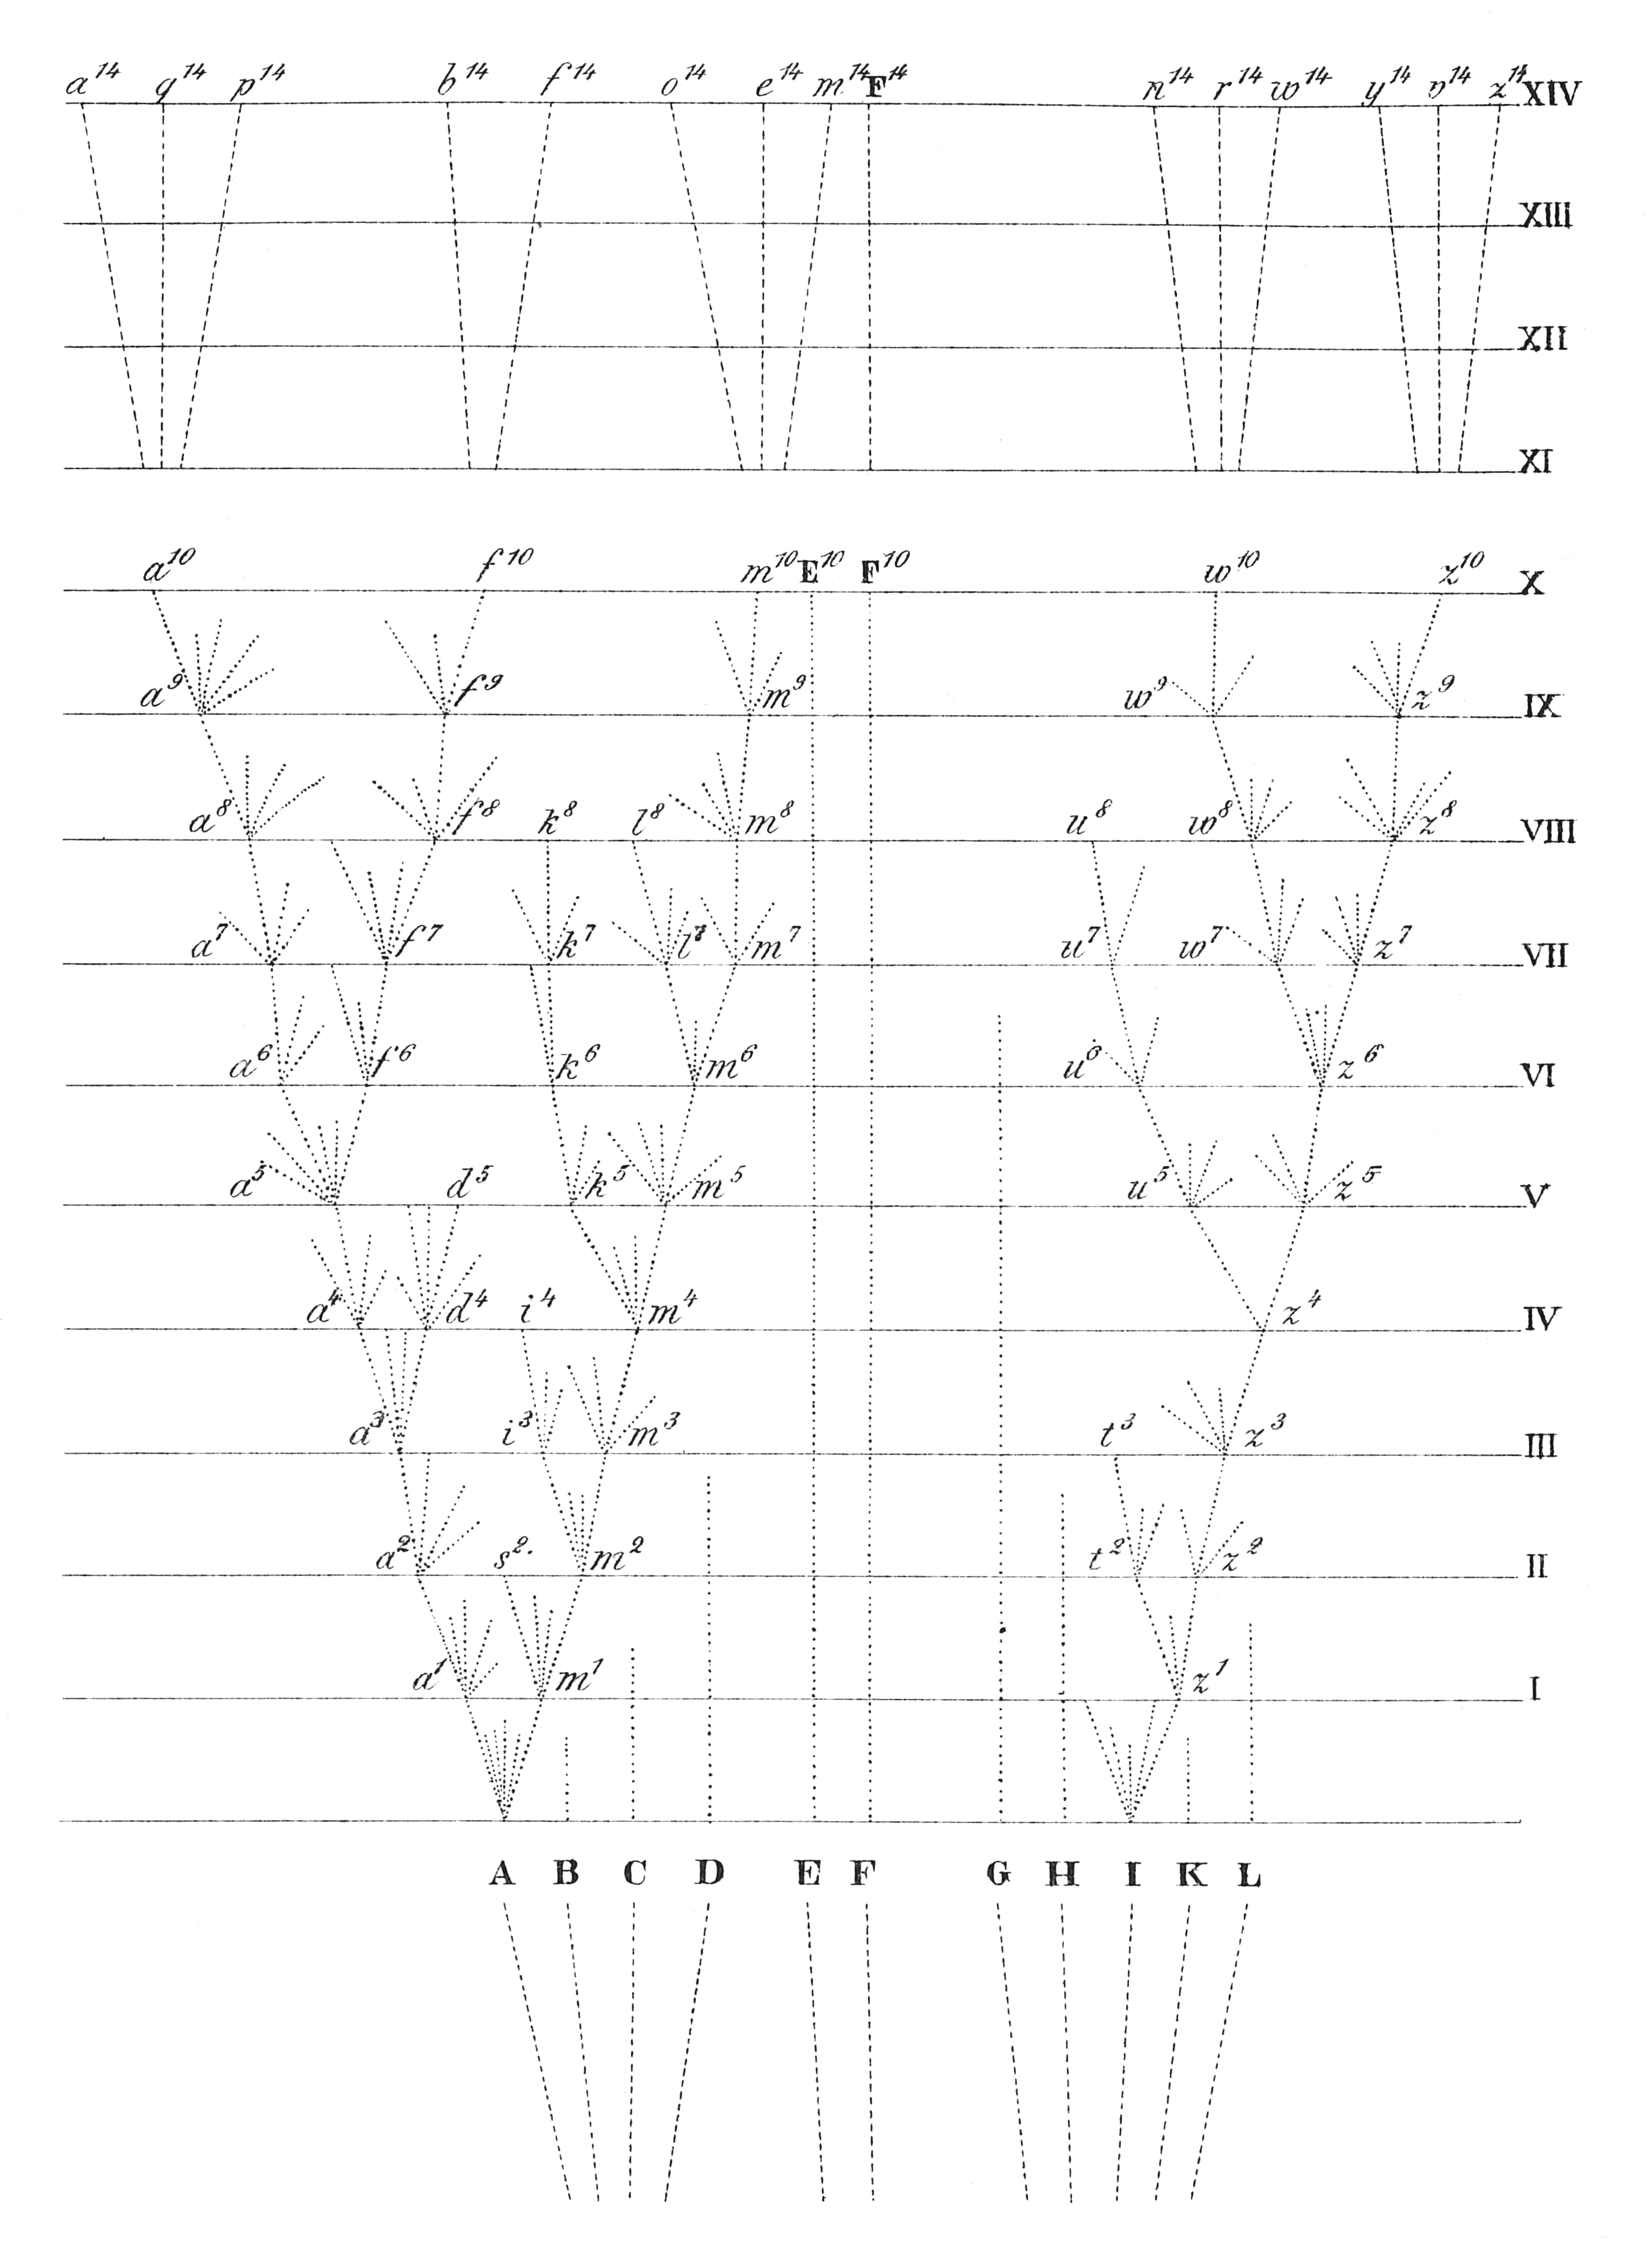
\includegraphics{bilder/plansch_1.png}
\label{fig:inverkan}
\end{figure}

framträder betydelsen af den grundsatsen, att en fördel är att härleda från karakterens divergens; ty denna skall leda dertill, att de mest skilda eller divergerande variationer (representerade af våra punkterade linier) bibehållas och ökas genom det naturliga urvalet. Då i vårt schema en af de punkterade linierna når en af de horisontala och der betecknas med en liten numererad bokstaf, så antages att variationen blifvit ökad till ett sådant omfång, att deraf bildats en distinct varietet, värd att upptagas i ett system.

Mellanrummen mellan två horisontala linier i figuren kunna motsvara 1000 generationer hvardera (bättre vore måhända tiotusen). Efter tusen generationer har arten A alstrat två väl utpräglade varieteter a${}^1$ och m${}^1$. Dessa två varieteter lefva fortfarande under samma yttre omständigheter som gjorde deras stamfäder föränderliga och benägenheten för föränderlighet är hos dem ärftlig; de skola följaktligen allt framgent vara benägna att variera och göra det också i allmänhet på ungefär samma sätt som deras stamfäder. Då dessa två varieteter vidare äro blott obetydligt modifierade former, hafva de äfven en viss böjelse att ärfva de fördelar, som gjorde deras föräldrar talrikare än de flesta andra invånare i samma trakt; de få äfven del af de mera allmänna fördelar, som gjorde det slägte hvartill stamfäderna hörde till ett i sitt eget land stort slägte. Alla dessa omständigheter äro, som vi veta, gynsamma för alstrandet af nya varieteter.

Om således dessa två varieteter äfven äro föränderliga, så skola i allmänhet de mest divergerande af deras variationer ega bestånd under de nästföljande tusen generationerna, och efter denna tids förlopp har varieteten a${}^1$ i schemat gifvit upphof till varieteten a${}^2$, hvilken enligt grundsatsen om divergensen bör visa större afvikelser från A än varieteten a${}^1$ gjorde. Vi antaga vidare att varieteten m${}^1$ har lemnat två varieteter nämligen m${}^2$ och s${}^2$, som skilja sig betydligt från hvarandra och i hög grad från det gemensamma ursprunget A. Samma process kunna vi följa steg för steg under huru lång tid som helst: några af dessa varieteter hafva efter hvarje tusental af generationer bildat en enda mer eller mindre afvikande varietet, andra två eller tre varieteter och andra åter ingen enda. Varieteterna eller de modifierade afkomlingarna som härstamma från det gemensamma ursprunget A tilltaga alltjemt i antal med divergerande karakter. I schemat är denna process fortsatt till den tiotusende generationen och i mera sammandragen och förenklad form till den fjortontusende.
Här vill jag dock anmärka, att processen icke alltid försiggår så regelbundet, som schemat föreställer, ehuru den äfven der synes något irregulier; det är sannolikt att hvarje form under lång tid blir oförändrad och sedan åter börja variera. Ej heller är det min åsigt att de mest divergenta varieteter utan undantag äro de som få väldet och föröka sig; en mellanform kan ofta ega bestånd en lång tid och stundom alstra en eller flera modifierade afkomlingar, stundom icke, ty det naturliga urvalet arbetar alltid för att fylla de platser, som antingen äro tomma eller illa besatta af andra varelser, och detta beror på oändligt invecklade förhållanden. Men såsom en allmän regel kunna vi uttala den satsen, att ju mer olika i skapnad ättlingarna af en art kunna blifva, ju flera platser i naturens hushållning äro de i stånd att intaga och i samma mån förökas deras modifierade afkomma. I vårt schema är successionslinien på regelbundna afstånd afbruten af små numererade bokstäfver, som beteckna de former hvilka varit tillräckligt skilda för att anses såsom varieteter. Men dessa afbrott äro imaginära och kunde inflätas hvar som helst på mellantider tillräckligt stora att medgifva en ansenlig grad af divergerande variation.

Då alla de modifierade ättlingarna af en gemensam, vidt utbredd art, tillhörande ett stort slägte, sträfva att få del af de fördelar som hafva gifvit deras stamfäder framgång i lifvet, skola de fortfarande tilltaga i antal och skilja sig i sina karakterer; detta betecknas i figuren genom antalet divergerande grenar utgående från A. De modifierade afkomlingarna från de sednare och mer förädlade grenarna i härstamningslinien skola sannolikt ofta intaga de tidigare och mindre förädlade grenarnas plats och således uttränga dem; detta betecknas i schemat derigenom att några af de lägre grenarna icke nå upp till de högre horisontala linierna. I några fall tviflar jag icke, att modifikationsprocessen är inskränkt till en enda härstamningsserie och att antalet ättlingar ej ökas, ehuru graden af divergens under de följande generationerna betydligt tilltagit. Detta fall skulle i schemat framställas om alla linierna, som utgå från A, vore borta med undantag af linien a${}^1$—a${}^{10}$. På sådant sätt hafva tydligen den Engelska ridhästen och den engelska rapphönshunden småningom i karakter skilt sig från sitt ursprung utan att hafva gifvit upphof till någon ny gren eller ras.

Efter tiotusen generationer antages arten A efterlemna tre former a${}^{10}$, f${}^{10}$ och m${}^{10}$, och då dessa under denna följd af generationer hafva i karakter aflägsnat sig från hvarandra, så skilja de sig nu betydligt, ehuru på olika sätt, både från hvarandra och från sitt gemensamma ursprung. Antaga vi graden af förändring emellan hvarje horisontal linie i vårt schema vara ytterligt liten, så hafva dessa former ännu blifvit blott väl markerade varieteter; men vi behöfva blott antaga dessa steg i modifikationsprocessen mera talrika eller större till omfång för att förvandla dessa tre former i tvifvelaktiga och slutligen väl bestämda arter; schemat visar således, huru små afvikelser, som utmärka varieteter, småningom steg för steg ökas till artskilnader. Om samma process fortgår under ett större antal generationer (såsom schemat visar i en sammanträngd och förenklad form), få vi åtta arter, utmärkta genom bokstäfverna a${}^{14}$—m${}^{14}$, alla härstammande från arten A. På detta sätt förökas enligt min åsigt arternas antal, och deraf bildas ett slägte.

Man kan antaga såsom sannolikt, att af ett stort slägte mer än en art varierar. I schemat har jag antagit, att en annan art I genom liknande stadier efter tiotusen generationer gifvit upphof till antingen två väl utpräglade varieteter eller två arter, alltefter den grad af förändring, som antages försiggå emellan två horisontala linier. Efter fjortontusen generationer antaga vi sex nya arter hafva bildats, betecknade med bokstäfverna n${}^{14}$—z${}^{14}$. I stora slägten är benägenheten att efterlemna ett stort antal modifierade ättlingar större hos de arter som från början äro mest skilda i karakter från hvarandra, ty dessa hafva största utsigten att fylla nya och vidt skilda platser i naturens hushållning; i schemat har jag derföre valt de långt skilda arterna A och I såsom de mest varierande och låtit dem bilda nya varieteter och arter. De andra nio arterna af vårt ursprungliga slägte, utmärkta med stora bokstäfver, kunna under en lång period efterlemna en oförändrad afkomma och detta har jag i schemat visat genom de punkterade linierna, som af brist på utrymme ej fortsatts långt uppåt.

Men under denna modifikationsprocess som schemat framställer har en annan af våra grundsatser spelat en stor rol, nämligen grundsatsen om tillintetgörelse. Då i hvarje fullt befolkad trakt det naturliga urvalet nödvändigt verkar derigenom, att de utvalda formerna hafva någon fördel öfver de andra i kampen för tillvaron, så måste de förädlade ättlingarna af en art hafva en beständig benägenhet att ersätta och undantränga sina föregångare och sina stamfäder. Ty vi få komma ihåg att kampen är i allmänhet häftigast emellan de former, som i kroppsbygnad, organisation och lefnadsvanor stå hvarandra närmast. Alla mellanformer emellan tidigare och senare stadier, det är emellan de mindre och mera förädlade stadierna af en art, likasom äfven den ursprungliga arten sjelf visa derföre i allmänhet benägenhet att dö ut. Detta är sannolikt förhållandet med många hela sidolinier, som besegras af nyare och mera förädlade linier. Likväl, om någon modifierad ättling af en art försättes i en särskild trakt eller plötsligt lämpar sig för någon viss ny station, i hvilken föräldrar och barn icke komma i någon täflan, så kunna båda fortfarande ega bestånd.

Om derföre vårt schema antages representera en hög grad af modifikation, så har arten A och alla tidigare varieteter dött ut och ersatts af åtta nya arter (a${}^{14}$—m${}^{14}$) och I har blifvit ersatt af sex (n${}^{14}$—z${}^{14}$) nya arter.

Men vi kunna gå ännu längre. De ursprungliga arterna af vårt slägte antogos likna hvarandra i olika grad, såsom förhållandet vanligen är i naturen; arten A står i närmare samband med arterna B, C och D än med de andra och arten I är närmare beslägtad med G, H, K, L än med de öfriga. Dessa två arter antogos också vara mycket allmänna och vidt utbredda, så att de ursprungligen måste hafva haft någon fördel öfver de flesta andra arterna af samma slägte. Deras modifierade ättlingar, fjorton till antal efter fjortontusen generationer hafva sannolikt ärft några af dessa företräden: de hafva också blifvit modifierade och förädlade på olika sätt i hvarje fortplantningsstadium, så att de blifvit lämpliga att innehafva många roler i deras hemlands naturhushållning. Det synes mig derföre ytterst sannolikt, att de hafva intagit just de ställen, som innehades icke blott af stamfäderna A och I utan äfven af några af de ursprungliga arterna, som närmast liknade deras stamfäder, och på detta sätt hafva de undanträngt dem. Helt få af de ursprungliga arterna skola derföre lemna efterkommande intill fjortontusende generationen, och vi kunna antaga, att blott en, F, af de två arter, som hade minsta likhet med de andra nio, ursprungliga arterna, har lemnat ättlingar ända till detta sena stadium.

De nya arter i vårt schema, som härstamma från de ursprungliga elfva arterna, äro nu femton till antal. På grund af det naturliga urvalets sträfvan att göra karaktererna divergenta är graden af karakterskilnad emellan a${}^{14}$ och z${}^{14}$ mycket större än emellan de mest skilda af de elfva ursprungliga arterna. De nya arternas förhållande till hvarandra är dessutom mycket olika. Bland de åtta ättlingarna af A är sambandet störst emellan de tre som betecknas med a${}^{14}$, q${}^{14}$ och p${}^{14}$, ty de hafva i en senare period utgrenats från a${}^{10}$; b${}^{14}$ och f${}^{14}$ äro till en viss grad skilda från de förstnämnda tre arterna, ty de hafva i en tidigare period utgått från a${}^{5}$; och o${}^{14}$, e${}^{14}$ och m${}^{14}$ stå slutligen i nära samband med hvarandra, men då de hafva afskilt sig redan vid modifikationsprocessens början äro de vidt skilda från de fem andra arterna och kunna bilda ett subgenus eller till och med ett särskildt slägte.

De sex ättlingarna af I bilda två subgenera eller genera. Men då den ursprungliga arten I är vida skild från A, ty de stå nästan vid motsatta ändar af slägtet, så bli de sex afkomlingarna af I på grund af ärftligheten allena vida skilda från de åtta afkomlingarna af A; de två grupperna antagas dessutom hafva alltjemt divergerat i skilda riktningar. Mellanformerna, som förenade de ursprungliga arterna A och I, hafva också (och detta är en mycket vigtig sak) alla med undantag af F dött ut och icke lemnat några efterkommande. De sex nya arterna som härstamma från I och de åtta som utgått från A skola derföre kunna erhålla rangen af slägten eller till och med flockar (underfamiljer).

På detta sätt hafva, som jag tror, två eller flera slägten uppkommit genom härstamning med modifikation från två eller flera arter af samma slägte, och de två eller flera urarterna kunna antagas härstamma från någon art af ett tidigare slägte. Detta är betecknadt i vårt schema derigenom att de brutna linierna under de stora bokstäfverna konvergera gruppvis nedåt emot en punkt; denna punkt representerar en enda art, den antagna stammen till våra nya subgenera och slägten.

Här kunna vi hafva god anledning att dröja ett ögonblick för att reflektera öfver karakteren af den nya arten F${}^{14}$, hvilken antages hafva divergerat blott obetydligt i karakter och bibehållit formen af F antingen oförändrad eller med blott ringa förändring. I detta fall är dess förhållande till de öfriga fjorton nya arterna af en egendomlig och invecklad beskaffenhet. Då den härstammar från en form, som stod emellan de två stamarterna A och I, hvilka antagas nu vara utdöda och okända, måste den till en viss grad i sina karakterer utgöra ett mellanstadium emellan de två grupper som utgått från dessa arter. Men då dessa två grupper hafva alltjemt i karakter skilt sig från sina urfäders typ, så är den nya arten F${}^{14}$ icke direkt en mellanform emellan dem, utan emellan typerna för tvenne grupper och hvarje naturforskare bör ej hafva svårt att påminna sig något sådant exempel.

I schemat hafva vi hittills antagit hvarje horisontal linie representera ett tusen generationer, men vi kunna lika väl låta dem föreställa millioner eller hundra millioner, och likaledes ett snitt af de på hvarandra liggande lagren af jordskorpan med de qvarlefvor af utdöda varelser de innehålla. Då vi komma till vårt kapitel om Geologien skola vi återkomma till detta ämne, och jag tror vi då skola finna, att detta schema sprider något ljus öfver de utdöda varelsernas slägtskap, hvilka, ehuru de i allmänhet tillhöra samma ordningar, familjer eller slägten som de nu lefvande, dock ofta till en viss grad i karakter stå emellan två existerande grupper; och vi kunna fatta detta förhållande, ty de utdöda arterna lefde på en mycket aflägsen tidpunkt, då ättlingarnas förgreningar ännu hade divergerat mindre från hvarandra.

Jag kan ej inse något skäl att begränsa den modifikationsprocess som vi nu genomgått till bildandet af slägten blott. Om vi i schemat antaga graden af variation, som representeras af hvarje grupp punkterade linier, vara mycket stor, bilda formerna a${}^{14}$—p${}^{14}$, b${}^{14}$—f${}^{14}$, och o${}^{14}$—m${}^{14}$ tre skilda slägten. Ifrån I hafva också utgått två skilda slägten, och då dessa senare två slägten både genom en fortsatt karaktersdivergens och genom arf från sitt ursprung skilja sig betydligt från de två slägten, som härstamma från A, så bilda de två små slägtgrupperna två skilda familjer eller till och med ordningar, alltefter graden af förändring som schemat antages föreställa. Och de två nya familjerna eller ordningarna hafva utgått från två arter af det ursprungliga slägtet och dessa två arter åter antagas härstamma från en art af ett ännu äldre okändt genus.

Vi hafva sett, att i hvarje trakt arterna af de större slägtena oftast erbjuda varieteter eller begynnande arter. Detta kunna vi i sjelfva verket vänta på förhand, ty då det naturliga urvalet verkar derigenom att en form har något företräde framför andra former i kampen för tillvaron, så verkar det hufvudsakligen på dem som redan hafva något företräde; och gruppens storlek bevisar att dess arter hafva ärft från en gemensam stamfar något gemensamt företräde. En täflan att lemna nya och modifierade ättlingar uppstår derföre emellan de större grupperna, som alla försöka att föröka sitt antal. En större grupp besegrar småningom en mindre, inskränker dess antal och förminskar på detta sätt dess utsigt till vidare variation och förädling. Inom samma stora grupp försöka de senare och mera fullkomliga undergrupperna, förgrenande sig och intagande många nya platser i naturens hushållning, att ersätta och tillintetgöra de tidigare och mindre förädlade undergrupperna; små enstaka grupper och undergrupper försvinna till slut helt och hållet. För framtiden kunna vi säga, att de grupper af organiska varelser, som nu äro stora och segerrika och äro minst afbrutna, det vill säga hafva undergått minsta förödelsen, skola under en lång tid alltjemt föröka sig. Men hvilka grupper till slut skola taga väldet, det kunna vi ej förutse, ty vi veta väl, att många grupper, som förr voro väl utvecklade, nu hafva helt och hållet gått ut. Se vi ännu längre in i framtiden, så kunna vi förutsäga, att en mängd smärre grupper skola helt och hållet utslockna och icke lemna några modifierade ättlingar på grund af de större gruppernas fortsatta och ständiga tillväxt, och att följaktligen af de arter som lefva på en viss period högst få lemna efterkommande in i en aflägsen framtid. I kapitlet om klassificering skall jag återkomma till detta ämne, jag vill blott tillägga, att med dessa satser, att ytterst få af de äldre arterna hafva efterlemnat afkomlingar och att alla ättlingarna af samma art bilda en klass, med dessa satser kunna vi lätt inse orsaken hvarföre i hvarje hufvudafdelning af växt- och djurriket blott ett ringa antal klasser finnas. Ehuru ytterst få af de äldsta arterna nu hafva lefvande och modifierade ättlingar, så måste dock jorden äfven i den mest aflägsna geologiska period hafva varit lika väl befolkad med många arter af många slägten, familjer, ordningar och klasser, som i närvarande tid.



\section{Framåtskridande i organisation.}

Det naturliga urvalet verkar såsom vi hafva sett uteslutande genom bevarande och samlande af sådana afvikelser, som kunna vara af nytta för en varelse under de organiska och oorganiska lefnadsvilkor, hvaraf den under succesiva perioder är beroende. Resultatet blir att hvarje varelse alltid sträfvar att förbättras i förhållande till dess lefnadsvilkor. Denna förbättring bör oundvikligen föra till den allmänna fulländning i organisation, som iakttages hos flertalet af de på jordytan utbredda varelserna. Här komma vi dock in på ett mycket svårt ämne, då ännu ingen naturforskare gifvit en allmänt tillfredsställande definition på hvad som förstås med organisationens fulländning. Hos ryggradsdjuren kommer härvid äfven med i räkningen deras själsförmögenheter och kroppsbygnadens större eller mindre likhet med menniskans. Man skulle tro, att graden af de förändringar, som de olika delarna och organerna undergått under sin utveckling från embryonaltillståndet intill mogen ålder, skulle kunna tjena såsom hållpunkt vid jemförelsen; dock förekomma fall, såsom vid de parasitiska krustaceerna, der flera delar af kroppen blifva ofullkomligare, så att man icke kan kalla det fullmogna djuret fullkomligare än dess larv. Von Baer’s måttstock synes ännu vara den bästa och allmännast användbara, nämligen graden af de olika delarnas differentiering (”i mogen ålder” torde väl få tilläggas) och deras speciela lämplighet för vissa förrättningar, eller fullständigheten af det fysiologiska arbetets fördelning, såsom Milne Edwards skulle säga. Huru dunkel denna sak ännu är, se vi dock om vi betrakta fiskarna till exempel, bland hvilka många naturforskare anse för de högsta dem som mest närma sig reptilierna, såsom hajarna, under det andra tillerkänna högsta platsen åt de vanliga benfiskarna (Teleostei), emedan de hafva den mest utbildade fiskformen och mest afvika från alla andra vertebrater. Ännu tydligare inse vi svårigheterna om vi vända oss till växterna, der den måttstock själsförmögenheterna kunna lemna helt och hållet bortfaller; några botanister ställa högst de växter, som i hvarje blomma hafva fullständigt utvecklade foderblad, kronblad, pistiller och ståndare, under det andra med större skäl anse för de fullkomligaste de växter, hvilkas olika organer äro starkare metamorfoserade och reducerade till mindre antal.

Taga vi de olika organernas differentiering och specialisering såsom bästa måttstocken för fullkomligheten af formernas organisation i fullväxt tillstånd (hvilket äfven innefattar hjernans fortgående utveckling för själsfunktionerna), så måste det naturliga urvalet uppenbarligen leda till fullkomlighet; ty alla fysiologer medgifva, att organernas specialisering, så vida de i detta tillstånd bättre fylla sin uppgift, är för hvarje organism en fördel, och det naturliga urvalet har således till ändamål att samla afvikelser som leda till organernas specialisering. I följd af den omständigheten, att alla organiska varelser sträfva att föröka sig i en hastigt växande progression och att intaga hvarje illa besatt plats i naturens hushållning, är det å andra sidan äfven möjligt, att det naturliga urvalet försätter en organisk varelse i sådana förhållanden, som göra många organer onyttiga eller öfverflödiga för honom och i sådant fall går han ett steg tillbaka i organisationsskalan. Om organisationen på det hela taget sedan de äldsta geologiska perioderna gått framåt ända till nu, det är en fråga, som lämpligare afhandlas i vårt kapitel om de organiska varelsernas geologiska succession.

Häremot kan man såsom invändning uppställa följande fråga: om alla organiska varelser allt ifrån början sträfvat att stiga högre och högre i utvecklingsskalan, hvaraf kommer det då, att på hela jordens yta ännu finnes en mängd de ofullkomligaste väsenden, och att i hvarje klass några former äro vida högre utvecklade än de andra? och hvarföre hafva icke dessa högre utbildade former redan öfverallt undanträngt och ersatt de mindre fullkomliga? Lamarck, som trodde på en medfödd och oundviklig benägenhet till fulländning hos alla organismer, synes hafva så väl känt vigten af denna invändning, att han ansåg sig nödgad till det antagandet, att enkla former alltjemt födas nya genom generatio spontanea (sjelfalstring). Jag behöfver icke säga, att vetenskapen på dess närvarande ståndpunkt icke lemnar något stöd för ett sådant antagande, att lefvande varelser någonstädes skulle uppstå af oorganisk materia. Enligt min teori erbjuder tillvaron af lägre organiserade djur ingen svårighet, ty det naturliga urvalet innefattar dock ingen nödvändig och allmän lag om framåtgående utveckling; det naturliga urvalet begagnar blott sådana förändringar, som för hvarje varelse äro af nytta i dess invecklade lefnadsförhållanden. Och nu kan man fråga: hvilken fördel skulle (så vidt vi kunna döma) ett infusionsdjur, en inelfsmask, eller till och med en daggmask hafva af en högre organisation? Hafva de ingen fördel deraf, så blifva de också föga eller intet fullkomligare genom det naturliga urvalet och förblifva således för oändliga tider stående på sin låga organisationsgrad. I sjelfva verket lär oss geologien, att några af de lägsta infusorier och rhizopodier sedan omätliga tider stått på samma utvecklingsgrad som nu. Det oaktadt skulle det vara förhastadt att antaga, att de flesta nu existerande lägre formerna sedan första början af sin tillvaro icke hade undergått någon förändring till fullkomlighet, ty hvarje naturforskare, som undersökt dessa organismer, hvilka nu betraktas såsom de lägsta på naturens stege, måste ofta förvåna sig öfver deras underbara och herrliga organisation.

Ungefär samma anmärkningar kunna göras med afseende på den stora olikheten i organisationsgrad inom hvarje större grupp, till exempel vid däggdjurens och fiskarnas samtidiga existens bland ryggradsdjuren, menniskans och näbbdjurets (Ornithorhynchus) bland däggdjuren, hajen och Amphioxus bland fiskarna; den sistnämde står i organernas enkelhet helt nära de ryggradslösa djuren. Men däggdjur och fiskar råka näppeligen i täflan med hvarandra; den höga ställning vissa däggdjur eller hela klasser intaga på högsta stadiet af organisation skall icke föranleda dem att intaga fiskarnas plats och på detta sätt undantränga dem. Fysiologerna tro, att hjernan måste matas med varm blod för att kunna utveckla sin högsta verksamhet och dertill är luftrespiration nödvändig, så att varmblodiga däggdjur som lefva i vatten i vissa hänseenden äro mera vanlottade än fiskarna. Likaså skola inom denna klass medlemmar af hajfamiljen sannolikt icke vara benägna att intaga Amphioxi plats, ty denna har, såsom jag hör af Fritz Müller, på södra Brasiliens magra och sandiga stränder en enda följeslagare och medtäflare, en anomalt bildad annelid. De tre lägsta däggdjursordningarna, pungdjuren, de tandlösa (trögdjuren) och gnagarna lefva i Sydamerika i samma trakter tillsammans med talrika apor och de störa hvarandra sannolikt föga. Ehuru organisationen i det stora hela kan vara stadd i framåtskridande, så måste dock utvecklingsskalan ännu framvisa alla grader, ty den höga utvecklingen hos vissa klasser eller enstaka medlemmar deraf leder ingalunda till totalt utslocknande af de grupper, med hvilka de icke komma i häftigare täflan. I några fall synas, såsom vi framdeles få se, lågt organiserade former hafva bibehållit sig ända till nu derföre att de haft egendomliga eller särskilda boningsorter, der de icke varit utsatta för någon starkare täflan, och derföre att de funnits till blott i ringa antal, hvilket enligt föregående reflexioner förminskar uppträdandet af gynsamma variationer.

Till slut tror jag, att de talrika, lågt organiserade formernas tillvaro på hela jordytan ibland nästan alla klasser beror på särskilda omständigheter. I vissa fall torde det hafva varit brist på fördelaktiga afvikelser, på hvilka det naturliga urvalet kunde hafva utöfvat sin verksamhet. I intet fall har väl tiden varit tillräcklig för att åstadkomma den högsta grad af utveckling; i några få fall kan äfven en så kallad ”organisationens återgång” hafva inträdt. Men hufvudorsaken ligger i den omständigheten, att under mycket enkla lefnadsomständigheter en högre organisation vore utan nytta, kanske till och med ofördelaktig, emedan den är finare, ömtåligare och lättare att störa och skada.

Ännu en invändning, som är rakt motsatt de nyss nämda har man framstält i följande fråga: om vi blicka tillbaka på lifvets första uppvaknande, då alla organiska varelser, såsom vi väl kunna föreställa oss, ännu egde den enklaste organisation, huru kunde då de första stegen till fulländning, differentiering och specialisering begynna? Herbert Spencer skulle sannolikt svara, att såsnart de enklaste encelliga organismer genom tillväxt och delning blifvit flercelliga eller fästat sig på någon yta, så skulle hans lag träda i verksamhet, att nämligen ”homologa enheter af hvilken ordning som helst differentieras i samma mån, som deras förhållande till på dem verkande krafter blir olika”. Men då inga fakta härvid kunna gifva oss någon ledning så är hvarje speculation i detta ämne onyttig. Det vore dock en villfarelse att antaga, att någon kamp för tillvaron och följaktligen något naturligt urval icke kunnat existera förr än många former först hade uppträdt. förändringar af en enda art på en afskild lokal kunna hafva varit fördelaktiga och genom sitt bestånd antingen omgestaltat hela arten eller gifvit upphof till två skilda former. Dock måste jag återkomma till hvad jag sagt redan vid slutet af inledningen, att ingen bör förundra sig, om ännu mycket angående arternas uppkomst måste förblifva oklart, då vi sväfva i fullkomlig ovisshet om jordinvånarnas ömsesidiga förhållande under så många förflutna perioder i deras historia.



\section{Granskning af åtskilliga invändningar.}

Jag vill nu granska några olikartade invändningar som man gjort emot mitt åskådningssätt, då några af de föregående frågorna härigenom skola blifva ytterligare belysta; att upptaga alla invändningar vore onyttigt, då sådana utgått från skriftställare, som icke gjort sig möda att riktigt förstå mina åsigter. Så har en utmärkt tysk naturforskare nyligen påstått, att den svagaste sidan af min teori ligger deri, att jag anser alla organiska varelser för ofullkomliga. Men jag har verkligen icke sagt annat, än att de alla i förhållande till de omständigheter under hvilka de lefva icke äro så fullkomliga som de kunde vara, och att detta är sant bevisa de många inhemska former, som på många delar af jorden afstå sina platser åt främmande naturaliserade inkräktare. Om också alla organiska varelser på någon tid vore fullkomligen lämpade efter sina lefnadsvilkor, så skulle de icke kunna förblifva lika fullkomliga, om dessa lefnadsvilkor långsamt ändrades; men ingen skall bestrida, att hvarje lands naturliga förhållanden liksom invånarnas antal och beskaffenhet äro underkastade ständiga vexlingar. Likaså antager en fransysk skriftställare i opposition mot hela detta arbetes anda, att enligt min åsigt stora och plötsliga förändringar träffat arterna, och frågar då triumferande, huru detta vore möjligt, då man ser att dylika modifierade former kunna kroaseras med de många oförändrade. Utan tvifvel blifva de små förändringarna eller afvikelserna beständigt störda eller tillbakahållna af kroaseringarna, med den så allmänna tillvaron af varieteter i samma land som stamarten lär, att kroasering icke nödvändigt förhindrar deras bildning, och för de vanliga lokala formerna eller geografiska raserna kan en kroasering alls icke komma i fråga. Man måste äfven komma ihåg, att affödan efter en kroasering emellan en modifierad och en icke modifierad art sträfvar att delvis ärfva båda föräldrarnas karakter och det naturliga urvalet skall helt säkert bevara till och med små tillstymmelser till nyttiga förändringar. Då dessutom en sådan kroaserad afföda har samma konstitution som den modifierade moderformen och är utsatt för samma yttre omständigheter, så skall den också lättare än andra individer af samma art undergå förändringar och modifieras på liknande sätt.

Man har framhållit, att då ingen af Egyptens kända växt- eller djurarter under de senaste tretusen åren förändrat sig, icke heller i andra verdsdelar några sådana förändringar hafva försiggått. De många djurarter, som sedan istidens begynnelse förblifvit oförändrade erbjuda en vida vigtigare invändning, ty de hafva varit utsatta för stora vexlingar i klimatet och de hafva nödgats att vandra öfver stora jordsträckor, under det i Egypten lefnadsvilkoren under de sista tretusen åren varit fullkomligt desamma. Detta från istiden lånade faktum kan väl framhållas emot dem som tro på tillvaron af en hos organismerna medfödd lag om nödvändig utveckling, men är kraftlöst emot läran om det naturliga urvalet, som blott antager, att inom en art afvikelser tillfälligtvis uppstå, och att dessa bevaras, om de äro fördelaktiga. Detta skall emellertid inträda blott efter långa tidrymder och efter förändringar i ett lands förhållanden.

Man har vidare framkastat denna fråga: då det naturliga urvalet är så verksamt, hvarpå beror det då, att icke det eller det organet i våra tider förändras och förbättras? hvarföre har icke honingbiets snabel blifvit så mycket förlängd, att biet kan suga nektar äfven i botten på rödklöfverns blommor? hvarföre har icke strutsen fått förmåga att flyga? Men antag att dessa organer hafva varierat i denna riktning, antag att trots kroasering och benägenhet till återgång tiden räckt till för det naturliga urvalets långsamma verksamhet, hvem vågar då påstå sig känna någon organisk varelses naturhistoria tillräckligt för att angifva hvilken särskild förändring skulle lända honom till nytta? Kunna vi till exempel med säkerhet säga, att en lång snabel icke skulle vara hinderlig för biet vid honingens utsugande ur så många andra blommor? Kunna vi påstå, att icke en längre snabel på grund af utvecklingens vexelverkan äfven skulle fordra en förstoring af andra mundelar, som skulle vara hinderliga vid deras fina cellbygnader? Hvad strutsen beträffar, så inses lätt, att denna öknens fågel skulle behöfva en utomordentlig tillökning i sin dagliga ranson för att kunna framforsla sin stora och tunga kropp genom luften. Så föga öfverlagda invändningar äro dock knappt värda att vederläggas.
Den utmärkta palæontologen Bronn har vid slutet af sin tyska öfversättning af detta arbete framstält den frågan, huru enligt grundsatsen om naturligt urval en varietet kan lefva jemte sin stamart. Om båda hafva blifvit lämpade för obetydligt olika lefnadsvanor eller förhållanden, kunna de existera bredvid hvarandra, ehuru bland djuren, som fritt kroaseras och drifva omkring, varieteter synas vara nästan helt och hållet inskränkta till bestämda trakter. Men om vi åsidosätta polymorfa arter, hvilkas föränderlighet synes vara af en egendomlig beskaffenhet, och alla tillfälliga variationer, sådana som olikheter i storlek, albinism etc. så finnas de mera beständiga varieteterna så vidt jag kan döma förlagda på bestämda stationer, hög- eller lågland, torra eller fuktiga områden eller skilda trakter. Bronn framhåller också, att bestämda arter aldrig skilja sig från hvarandra blott i en enda karakter utan i många delar; och han frågar efter orsaken hvarföre det naturliga urvalet ovilkorligen samtidigt inverkar på många delar af organismen. Men det finnes icke den minsta nödvändighet att tro att alla delar hafva samtidigt blifvit modifierade; de hafva kunnat förvärfvas den ena efter den andra, och då de samtidigt gå i arf, synas de oss såsom samtidigt bildade. Vexelverkan bör dessutom förklara förändringar som flera delar undergå, då en viss annan del modifieras. Bevis härpå se vi i våra husdjursarter, som om de också i en viss utvald karakter afvika betydligt, alltid till en viss grad förete afvikelser äfven i andra karakterer.

Bronn frågar vidare, huru det naturliga urvalet kan förklara olikheter emellan arter, som tyckas vara af ingen fördel för dessa arter, såsom längden af öronen eller svansen eller emaljens veck i tänderna hos flera arter af harar och råttor. Hvad växterna beträffar har detta ämne nyligen blifvit behandladt i ett utmärkt arbete af Nägeli. Han medgifver att det naturliga urvalet har gjort mycket, men han påstår, att växtfamiljerna skilja sig från hvarandra hufvudsakligen i morfologiska karakterer, som synas alldeles oväsentliga för arternas bestånd. Han tror följaktligen på en medfödd tendens till fulländning eller fortgående utveckling. Han anför cellernas anordning i väfnaderna och bladens på stammen såsom momenter på hvilka det naturliga urvalet ej kan hafva något inflytande. Dertill kan läggas de numeriska delningarna af blommans delar, fröämnenas läge, fröens form så vida den icke är af nytta vid spridningen. Professor Weismann, som granskat Nägelis afhandling, förklarar sådana olikheter med beskaffenheten af organismen under vissa omständigheters inverkan, och detta är detsamma som jag har kallat lefnadsförhållandenas direkta och bestämda verkan, hvaraf alla eller nästan alla individer af samma art variera på samma vis. Om vi påminna oss sådana fall, som vissa monstrositeter, hvilka icke kunna förklaras med regress, eller dylikt, och sådana hastiga starkt markerade bildningsafvikelser, som uppträdandet af en mossros på en vanlig ros, måste vi medgifva, att individens organisation är i stånd att enligt sina egna utvecklingslagar under vissa vilkor undergå stora modifikationer, oberoende af det gradvisa hopandet af små ärfda förändringar. Åtskilliga morfologiska olikheter till hvilka vi framdeles återkomma, höra säkerligen under denna rubrik; men många olikheter kunna i närvarande tidpunkt vara af stor nytta, eller kunna under en förfluten tid hafva varit det, ehuru vi icke äro i stånd att fatta deras bruk, och derföre hafva de stått under det naturliga urvalets inflytande. Ett ännu större antal af morfologiska skiljaktigheter kunna säkerligen betraktas såsom ett nödvändigt resultat — genom tryck, brist eller öfverflöd på näring, genom en tidigare utvecklad dels inflytande på en sedermera tillkommen, vexelverkan etc. — af andra förändringar, som alla arter måste hafva genomgått under den långa modifieringsprocessen.

Ingen vill väl påstå, att vi hittills känna bruket af hvarje del af någon växt eller funktionen af hvarje cell i ett nytt organ. För fem eller sex år sedan skulle en mängd besynnerligheter i bildningen af orchideernas blommor, stora kammar och balkar och de olika delarnas relativa läge hafva betraktats såsom onyttiga morfologiska olikheter, men nu veta vi att de äro af stor nytta och måste hafva lydt under det naturliga urvalets verksamhetsområde. Ingen kan för närvarande förklara, hvarföre bladen i en spira med hvarandra bilda vissa vinklar, men vi kunna se, att deras anordning står i sammanhang med deras afstånd från bladen på alla sidor omkring dem, och vi kunna med skäl hoppas få ett bevis, att vinklarna bero på någon sådan orsak, som tillkommandet af nya blad till den hopträngda spiran i knoppen, likasom vinklarna i biens celler ovilkorligen bero af det sätt hvarpå insekterna arbeta tillsammans.

I vissa hela grupper af växter stå fröämnena upprätta och i andra äro de hängande, och hos några få växter intaga inom samma fruktämne några frön den ena och andra den andra ställningen. Dessa lägen synas först vara rent morfologiska och icke af någon fysiologisk betydelse, men Hooker har meddelat mig, att af fröen inom samma fruktämne i några fall blott de öfre, i andra fall blott de nedre befruktas, och han förmodar, att detta sannolikt beror på den riktning i hvilken pollenröret intränger. Om detta är förhållandet, så kan fröämnenas läge, äfven om det ena är upprätt och det andra hängande, vara en följd af urval af någon ringa afvikelse i läge som kunde gynna deras befruktning och frösättning.

Flera växter, som höra till skilda ordningar, frambringa vanligen blommor af två slag, dels öppna och af vanlig skapnad, dels slutna och ofullkomliga. I de senare äro kronbladen nästan alltid reducerade till blotta rudimenter och pollenkornen äro förkrympta; i ståndarstammarna hos Ononis äro skiftevis fem ståndare rudimentära och hos några arter af Viola äro tre ståndare af denna beskaffenhet och de två öfriga behålla sin funktion, men äro mycket små. I sex bland trettio af de slutna blommorna hos en indisk viol (namnet okändt, emedan den hittills icke gifvit några fullkomliga blommor) voro foderbladen reducerade från det normala antalet fem till tre. I en grupp af Malpighiaceæ äro enligt A. de Jussieu de slutna blommorna ännu mera modifierade, ty de fem ståndare som stå midt emot foderbladen äro alla felslagna och den sjette som står emot ett kronblad är ensam utbildad; denna ståndare saknas deremot i de vanliga blommorna af dessa arter; stiftet saknas och fruktämnena äro reducerade från tre till två. I alla dessa växter äro de slutna blommorna af synnerlig nytta, ty med fullkomlig säkerhet och med en ytterst ringa mängd frömjöl lemna de en riklig mängd frön, under det de fullt utbildade blommorna tillåta tillfälliga kroaseringar med andra individer. Dessa förändringar kunna derföre vara och äro otvifvelaktigt följder af ett naturligt urval, och jag kan tillägga att nästan alla gradationer emellan fullkomliga och ofullkomliga blommor stundom kunna iakttagas hos samma växt.

Utrymmet tillåter blott några få belysningar öfver de modifikationer, som ovilkorligen följt från andra förändringar, genom brist eller öfverflöd på näring, genom tryck eller andra okända orsaker. Hos den spanska kastanien och vissa furuträd skilja sig bladens divergensvinklar enligt Schacht på de horisontala och de uppräta grenarna. Hos den vanliga vinrutan och några andra växter öppnar sig en blomma först, vanligen den centrala eller terminala, och har fem foderblad och kronblad och femrummigt fruktämne, under det de andra blommorna på växten äro fyrtaliga. Hos den britiska Adoxa har den öfversta blomman vanligen två foderflikar med de öfriga organerna fyrtaliga, under det de omgifvande blommorna hafva tre foderflikar och de öfriga blomdelarna femtaliga, och denna olikhet synes bero af det sätt, hvarpå blommorna äro packade tillsammans. Hos många Compositæ och Umbelliferæ och några andra växter hafva de periferiska blommorna sina kronor vida mera utvecklade än de centrala, och detta är sannolikt en följd af naturligt urval, ty alla blommorna blifva på detta sätt mera märkbara för de insekter som äro nyttiga eller nödvändiga till deras befruktning. I förening med blomkronans större utveckling äro reproduktionsorganerna mer eller mindre felslagna. Det är ett egendomligt förhållande att skalfrukterna vid omkretsen stundom skilja sig från dem i centrum genom form, färg och andra karakterer. Hos Carthamus och några andra Compositæ äro blott de centrala frukterna försedda med fjun, och af Hyoseris lemnar samma hufvud frukter af tre olika former. Hos vissa Umbelliferæ äro enligt Tausch de yttre frukterna orthosperma, de inre coelosperma, och denna skilnad har af de Candolle betraktats såsom af den högsta systematiska betydelse inom familjen. Om i sådana fall som föregående alla blad, blommor, frukter etc. på samma växt hade underkastats samma yttre och inre förhållanden, skulle utan tvifvel alla hafva visat samma morfologiska karakterer, och det skulle tydligen icke varit af nöden att åberopa grundsatsen om fortgående utveckling. För de små slutna blommorna, äfvensom många lägre parasitdjur, om det antages, att ett sådant biträde behöfves, måste vi åberopa en medfödd tendens till återgående utveckling.

Många exempel kunde gifvas på morfologiska karakterer som visa en höggradig föränderlighet hos växter af samma art, hvilka växa nära tillsammans, eller till och med på samma växtindivid, och några af dessa karakterer betraktas såsom systematiskt ovigtiga. Jag vill blott anföra några få fall, som jag först påträffade. Jag behöfver icke framhålla några exempel af blommor på samma stånd med dels fyrtaliga, dels femtaliga blomdelar; jag vill nämna, att enligt de Candolle blommorna af Papaver bracteatum hafva två foderblad och fyra kronblad (hvilket är vanliga förhållandet hos vallmo) eller tre foderblad och sex kronblad. Kronbladens läge i knoppen är i de flesta grupper en konstant morfologisk karakter, men professor Asa Gray försäkrar, att hos några arter af Mimulus kronbladens läge lika ofta öfverensstämmer med förhållandet hos Rhinantideæ som Antirrhineæ, till hvilken grupp slägtet hör. August S:t Hilaire anför följande fall: slägtet Xanthoxylon hör till en afdelning af Rutaceæ med enkelt fruktämne, men hos några arter finnas blommor på samma växt, till och med i samma vippa, med ett eller två fruktämnen. Hos Helianthemum har frökapseln beskrifvits såsom en- eller trerummig, och hos H. mutabile ”une lame plus ou moins large s’étend entre le pericarpe et le placenta”. Slutligen fann S:t Hilaire af Gomphia oleæformis emot sydligaste delen af dess utbredningsområde två former, hvilka han först utan betänkande antog för skilda arter, men sedan såg växa på samma buske, och han tillägger: ”Voilà donc dans un même individu des loges et un style qui se rattachent tantôt à un axe verticale et tantôt à un gynobase.”

Kan man säga om dessa växter, att de hafva blifvit påträffade under fortgåendet till en högre grad af utveckling? Tvärtom skulle jag från dessa karakterers rikliga variation sluta till, att de äro af ringa vigt för växten sjelf, huru stor betydelse de än må hafva för oss i våra klassifikationer. Ehuru vi äro fullkomligt okunniga om den verkande orsaken till hvarje modifikation, synes det likväl sannolikt af hvad vi känna om förhållandet emellan föränderligheten och förändring i lefnadsvilkoren, att under vissa förhållanden den ena bildningen haft öfvermagten öfver den andra och på detta sätt blifvit fullkomligt eller nästan konstant. Då sådana skiljaktigheter äro af ingen betydelse för artens välfärd, hafva de små afvikelser som uppkommit icke blifvit ökade eller samlade genom naturligt urval och de löpa fara att utplånas genom tillfälliga kroaseringar med andra individer. En bildning som utvecklats genom ett länge fortsatt urval blifver, då den icke längre är till någon tjenst för arten, i allmänhet föränderlig, såsom vi se förhållandet vara med de rudimentära organerna, ty den står icke längre under urvalets inflytande; men å andra sidan då i följd af organismens beskaffenhet eller förändring i de yttre förhållandena bestämda modifikationer hafva bildats, hvilka äro utan vigt för artens bestånd, kunna de öfvergå och hafva ofta öfvergått i nästan samma tillstånd till på annat sätt modifierade ättlingar. Hår hafva öfvergått på nästan alla däggdjur, fjädrar på alla fåglar och fjäll till alla reptilier. En bildning, hvilken den än må vara, som är gemensam för många beslägtade former anses af oss såsom af hög systematisk betydelse och antages på den grund ofta vara af hög fysiologisk vigt för arten. Morfologiska skiljaktigheter som vi anse för vigtiga — såsom bladens anordning, fruktämnets delning, fröämnenas läge etc. — uppträdde sannolikt först såsom vexlande variationer, som förr eller senare blefvo nästan konstanta i följd af organismens beskaffenhet eller de omgifvande förhållandena, samt genom kroasering; ty då dessa morfologiska karakterer icke hafva något inflytande på artens bestånd, så kunna små förändringar i dem icke begagnas och samlas af det naturliga urvalet. Det är ett egendomligt resultat vi sålunda kommit till, nämligen att karakterer af ringa vital betydelse för arten äro de vigtigaste för systematikern, men såsom vi skola se framdeles vid behandlingen af klassifikationens grundsatser, är denna paradox icke så stor som den först synes. Hvad man än må tänka om denna åsigt, i intet af de föregående exemplen lemna så vidt jag kan döma fakta något bevis för en medfödd tendens till fulländning eller fortgående utveckling.

Jag behöfver blott fästa mig vid två andra invändningar. Den utmärkta botanisten H. C. Watson anser mig hafva för högt uppskattat vigten af grundsatsen om karakterens divergens (på hvilken han dock uppenbart sjelf tror) och säger, att man äfven måste taga med i betraktande hvad man kunde kalla ”karakterens konvergens”. Detta är dock en allt för invecklad fråga, att vi skulle kunna inlåta oss på den här. Jag vill blott anmärka, att om två arter af två närstående slägten frambringa ett antal nya divergenta arter, kan jag väl föreställa mig, att några bland dem å ömse sidor så mycket närma sig hvarandra, att man för beqvämlighets skull kan sammanställa dem i ett intermediärt slägte, till hvilket alltså de två slägtena konvergera. Men i följd af ärftlighetsprincipens stränghet är det troligt, att dessa två grupper af nya arter åtminstone bilda två afdelningar i det nya slägtet.

Watson har äfven invändt, att det naturliga urvalets fortsatta verksamhet med karaktersdivergens slutligen måste föra till ett obegränsadt antal artformer. Hvad dock beträffar de blott oorganiska yttre lefnadsvilkoren, så är det väl sannolikt, att snart ett tillräckligt antal arter lämpar sig efter alla ansenligare olikheter i värme, fuktighet och så vidare; dock medgifver jag fullkomligt, att relationerna emellan de organiska varelserna äro vigtigare, och då arterna af de organiserade invånarna i en trakt beständigt föröka sig, så blifva äfven de organiska lefnadsvilkoren allt mera invecklade. På den grund synes det verkligen vid första påseende icke finnas någon gräns för mängden af nyttiga formolikheter och följaktligen icke för artantalet. Vi veta, att icke en gång de rikast befolkade områden på jordytan äro fullständigt försedda med arter; på Goda Hoppsudden och i Australien, som förete en förvånande mängd arter, hafva dock många europeiska arter blifvit naturaliserade. Geologien lär oss dock, att alltifrån den långa tertiärperiodens första tid antalet molluskarter icke betydligt eller alldeles icke tilltagit, liksom icke heller däggdjursarterna från mellersta tiden af samma period. Hvad är det då som förhindrar artantalets tillväxt i oändlighet? Summan af lif (jag menar icke antalet af artformer) på en gifven yta måste hafva en gräns, betingad af de fysiska förhållandena, så att om densamma är bebodd af många arter, hvarje eller i det närmaste hvarje art måste representeras af blott ett ringa antal individer och följaktligen löpa fara att tillintetgöras redan genom en tillfällig vexling i årstidernas beskaffenhet eller i antalet af fiender. En sådan förödelseprocess kan gå raskt för sig, under det arternas nybildning sker mycket långsamt. Antaga vi såsom ett fall af ytterlighet, att i England funnes lika många arter som individer, så skulle första stränga vinter eller torra sommar utrota tusen sinom tusen arter. Sällsynta arter (och hvarje art blir sällsynt, om antalet arter växer i oändlighet) lemna enligt vår ofta upprepade grundsats på en gifven tidrymd blott få fördelaktiga afvikelser och kunna således blott långsamt utveckla nya artformer. Blir en art mycket sällsynt, så måste äfven parningen emellan nära slägtingar medverka till deras undergång; åtminstone hafva några författare anfört denna omständighet såsom orsak till bisonoxens utgång i Lithauen, hjortens i Skottland, björnens i Norge och så vidare. Slutligen (och detta synes mig vara det vigtigaste), en dominerande art, som redan i sitt eget hemland öfvervunnit många medtäflare, skall alltid sträfva att vidare utbreda sig och ersätta andra. Alphonse de Candolle har visat, att de arter som sprida sig vida omkring vanligen sträfva efter mycket stor utbredning och således komma i tillfälle att på olika områden tillintetgöra mångfaldiga medtäflare och på detta sätt hindra de specifika formernas omåttliga tilltagande i verlden. Dr Hooker har nyligen visat, att på Australiens sydöstra spets, der tydligen många inkräktare från många verldstrakter finnas, de inhemska australiska arterna betydligt aftagit i antal. Jag tillåter mig icke att fråga, hvilken vigt bör läggas på alla dessa betraktelser, dock måste de i förening med hvar andra sätta en gräns för benägenheten till artformernas oändliga förökning.



\section{Sammanfattning af hela kapitlet.}

Om under den långa raden af tidsperioder och under vexlande yttre förhållanden de organiska varelserna variera i flera delar af organisationen, hvilket jag tror icke kan bestridas, om på grund af hvarje arts sträfvan att föröka sig i geometrisk progression en häftig kamp för tillvaron under någon period, årstid eller år måste utkämpas, och detta kan säkerligen icke bestridas, om vi taga i betraktande alla organiska varelsers invecklade förhållanden till hvarandra och till vilkoren för deras existens, som hafva till följd en oändlig för dem gynsam omvexling i kroppsbygnad, konstitution och lefnadsvanor, då tror jag, att det skulle synas högst egendomligt, om icke någon variation hade bildats, som varit nyttig för varelsens egen välfärd, då så många variationer förekommit som varit nyttiga för menniskor. Men om sådana för en organisk varelse gynsamma variationer förekomma, så hafva helt säkert de derigenom utmärkta individerna mesta utsigten att ega bestånd i kampen för tillvaron och enligt den stränga principen om ärftligheten sträfva de att lemna en lika utmärkt afföda. Denna grundsats om de gynsamt utrustade varelsernas bestånd har jag för korthets skull kallat det naturliga urvalet. Den leder till hvarje skapad varelses fullkomnande i förhållande till dess organiska och oorganiska lefnadsvilkor och följaktligen i de flesta fall till hvad man måste anse för organisationens fulländning; det oaktadt kunna lägre stående, enklare former länge hafva bestånd, om de äro väl lämpade för sina enklare lifsvilkor.

Enligt grundsatsen om egenskapers ärftlighet vid motsvarande ålder kan det naturliga urvalet modifiera ägget, ungen, likaväl som den fullväxta individen. Hos många djur bör det sexuela urvalet i sin verksamhet understödja det naturliga urvalet genom att tillförsäkra de starkaste och lämpligaste hannar största antalet afföda. Det sexuela urvalet kan äfven förläna sådana karakterer, som för hannarna allena äro af nytta i deras kamp med andra hannar.

Om nu det naturliga urvalet verkligen har i naturen medverkat till att modifiera och lämpa de särskilda lifsformerna efter deras olika förhållanden och lokaler, det måste bedömas efter värdet af de i de följande kapitlen gifna bevisen. Men vi se redan huru den verkar tillintetgörelse och i hvilken vidsträckt grad tillintetgörelsen varit verksam i jordens historia visar tydligt geologien. Det naturliga urvalet leder också till karakterens divergens, ty ju mer de organiska varelserna äro olika i kroppsbygnad och lefnadsvanor, ju flera kunna lefva på samma område, derpå se vi exempel om vi betrakta invånarna på en liten yta eller naturaliserade produkter. Under en arts modifikation, under alla arters oupphörliga bemödanden att föröka sitt antal, ju mera olika ättlingarna blifva, ju större är deras utsigt att segra i kampen för tillvaron. De små olikheter som utmärka varieteterna af samma art sträfva alltså ständigt att tilltaga, till dess de likna de större skilnaderna emellan arterna af samma slägte eller till och med emellan skilda slägten.

Vi hafva sett, att det är de vanliga, vidt utbredda arterna af de större slägtena som variera mest, och dessa sträfva att lemna i arf åt sina modifierade ättlingar denna öfverlägsenhet, som nu gör dem till de herskande i sina områden. Såsom vi nyss hafva anfört, leder det naturliga urvalet till karaktersdivergens och till utrotande af de mindre förädlade, intermediära lifsformerna. Från dessa grundsatser tror jag vi kunna förklara slägtskapen emellan alla organiska varelser af alla klasser på hela jordytan. Det är i sanning ett underbart faktum — ett under, som vi lätt förbise, då vi äro så förtrogna dermed — att alla djur och alla växter i alla tider och allestädes äro så beslägtade med hvarandra, att de bilda grupper, som äro subordinerade under andra grupper, så att såsom vi öfverallt finna varieteter af samma art äro mest beslägtade med hvarandra, arter af samma slägte visa mindre och olika slägtskap med hvarandra, bildande sectioner och subgenera, arter af skilda slägten äro ännu mindre beslägtade och slägtena med hvarandra stå i olika nära samband bildande underfamiljer, familjer, ordningar, underklasser och klasser. De olika underordnade grupperna i en klass kunna icke ordnas i en enkel serie utan synas snarare samla sig omkring vissa medelpunkter, och de deraf bildade grupperna åter omkring andra medelpunkter och så vidare i nästan oändliga cirklar. Från den åsigten att hvarje art blifvit särskildt skapad kan jag ej vänta någon förklaring af detta vigtiga faktum i alla organiska varelsers klassificering, men så vidt jag kan döma, kan det förklaras genom ärftlighet och genom den förenade verkan af naturligt urval, som verkar tillintetgörelse och karaktersdivergens, såsom vi i vårt schema hafva visat.

Slägtskapen emellan alla varelser af samma klass har stundom blifvit framstäld genom bilden af ett stort träd. Jag tror, att denna bild mycket nära motsvarar sanningen. De gröna och nyss utspruckna grenarna kunna föreställa nu existerande arter och de som bildats under föregående år hela raden af utdöda arter. Vid hvarje växtperiod hafva alla växande grenar försökt att förgrena sig åt alla håll och att skjuta öfver och undertrycka de omgifvande skotten och grenarna, på samma sätt som arter och artgrupper hafva försökt att i den stora kampen för tillvaron öfverväldiga andra arter. De stora grenarna, fördelade i allt mindre och mindre grenar och qvistar, voro sjelfva en gång, då trädet var litet, nyss utskjutna grenar och denna förening emellan de tidigare och de nuvarande skotten genom grenar kan väl föreställa klassifikationen af alla utdöda och lefvande arter i grupper och underordnade grupper. Af de många telningar som utvecklade sig då trädet blott var en liten buske qvarstå blott två eller tre, nu utväxta till stora grenar, och dessa bära nu alla de andra mindre grenarna: så hafva också af alla de arter, som lefvat under förgångna geologiska perioder, blott få ännu lefvande och modifierade ättlingar. Från trädets första utväxt har mången gren vissnat och fallit af och dessa förlorade grenar af olika storlek kunna representera alla de ordningar, familjer och slägten, som icke hafva några nu lefvande representanter och hvilka vi känna blott genom fossilier. Liksom vi här och der se en enstaka svag gren utgå från en gaffeldelning långt ned på trädet och genom någon lycklig slump ännu lefva qvar ända till dess spets, så se vi stundom ett djur, såsom Ornithorhynchus eller Lepidosiren, hvilket i någon ringa grad genom sina slägtskapsförhållanden förenar två större grupper, och hvilket tydligen blifvit räddadt undan en olycksbringande strid, derigenom att det bebott något skyddadt område. På samma sätt som knoppar genom tillväxt gifva upphof till nya knoppar och dessa, om de äro kraftiga, förgrena sig och på alla håll skjuta öfver mången svagare gren, så tror jag det har varit förhållandet med det stora lifsträdet, som med sina döda och afbrutna grenar fyller jordskorpan och betäcker ytan med sina herrliga alltjemt vidare fortgående förgreningar.


